In this section we present a detailed computational study of the automated
goal-oriented adaptive algorithm presented in \autoref{sec:Algorithm} applied to
some time-dependent test problems. To this end we first we apply our algorithm
to a linear problem, first for a diffusion dominated problem,
\autoref{tst:ADRk1E-1}, and then for a convection dominated problem,
\autoref{tst:ADRk1E-5}.  Namely, we demonstrate the effectiveness of
\autoref{alg:Adaptivity} on the Advection-Reaction-Diffusion equation. Next we
demonstrate the effectiveness of \autoref{alg:Adaptivity} on non-linear
problems, where the error representation is no longer orthogonal. To this end,
we apply the algorithm to a benchmark problem presented in Sch\"afer et
al.\cite{Schaefer1996}, \autoref{tst:Drag} and \autoref{tst:Velocity}, where the
equation of interest is the Icompressible Navier-Stokes equation and our
particular focus is on flow around a bluff body.  Finally, in
\autoref{tst:rhoNSE}, we apply our algorithm to the ever more complex problem of
Variable Density Incompressible Navier-Stokes equation, where we focus on the
solution to Rayleigh-Taylor instability.

For each test below we set the max number of iterations to $25$ and set the
$TOL=-1$. In this way we will treat the solution obtained from the final
adaptive mesh as the so-called 'true solution' and use this solution to
determine the effectivity of the adaptive algorithm.

\subsection{Linear Problems}
    In this subsection we demonstrate the effectiveness of
    \autoref{alg:Adaptivity} on linear PDEs. That is, we demonstrate that
    \autoref{alg:Adaptivity}, performs better than the uniform refinement for
    linear problems. To that end we apply the adaptive algorithm to
    the Advection-Reaction-Diffusion equation (ARD).

\subsubsection{Advection-Reaction-Diffusion Equation} \label{sss:ADR}
    The ARD is a simple linear model of a reactive and diffusive flow.  In what
    follows the parameters $\alpha,\,\beta$, and $\kappa$ represent the
    reactivity, convective velocity vector, and diffusivity tensor,
    respectively. Thus, for $t\in [0,T]$ and a domain $\Omega$ with boundary
    $\partial \Omega$, the ARD is given by
    \begin{equation}
        \begin{split}
            u_t + \nabla \left(\kappa\cdot \nabla u \right) + \beta \cdot \nabla
                u + \alpha u = f,& \quad \mathbf{x} \in \omega, \\
            u = g,& \quad \mathbf{x} \in \partial \omega, \\
            u = 0,& \quad t = 0,\, \mathbf{x} \in \partial \omega,
        \end{split}
        \label{eq:ADR}
    \end{equation}
    where $f$ is the external forcing.

    For this particular example we take the domain to be a square domain with a
    center square removed. That is we take the outer square to be $\Omega_1$ and
    the inner square to be $\Omega_2$ and the resulting domain $\Omega$ is given
    by
    \begin{equation}
        \Omega = \Omega_1\setminus \Omega_2,
        \label{eq:ADRDomain}
    \end{equation}
    and then the boundary $\partial \Omega$ is defined as
    \begin{equation}
        \partial \Omega = \partial \Omega_1 + \partial \Omega_2,
        \label{eq:ADRBoundary}
    \end{equation}
    where $\partial \Omega_1$ is the boundary of $\Omega_1$ and $\partial
    \Omega_2$ is the boundary of $\Omega_2$ (see \autoref{fig:ADRDomain}.

    \begin{figure}[h]
        \centering
        \tikzstyle{next}=[->, thick, shorten <=1pt, shorten >=1pt]
        \begin{tikzpicture}[scale=6]
            \draw (0,0) -- (1,0) -- (1,1) -- (0,1) -- cycle;
            \draw (0.4,0.4) -- (0.6,0.4) -- (0.6,0.6) -- (0.4,0.6) -- cycle;
            \node (Omega_2) at (0.5,0.5) {$\Omega_2$};
            \node (dOmega_2) at (0.5,0.65) {$\partial\Omega_2$};
            \node (Omega_1) at (0.25,0.25) {$\Omega_1$};
            \node (dOmega_1) at (0.5,0.05) {$\partial\Omega_1$};
        \end{tikzpicture}
        \caption{Problem Geometry, $\Omega$, for ARD small hole problem.}
        \label{fig:ADRDomain}
    \end{figure}

    Furthermore, in this example we will take the subdomains to be $\Omega_1 =
    [0,1]^2$ and $\Omega_2 = [0.48,0.52]^2$. With these subdomains defined we
    take the boundary condition to be
    \begin{equation}
        g = \begin{cases}
            0   &\mathbf{x} \in \partial \Omega_1 \\
            5 + 5\, \sin \pi\, t  &\mathbf{x} \in \partial \Omega_2
        \end{cases}.
        \label{eq:ADRBCs}
    \end{equation}
    Finally we take the final time $T=10,\, \alpha=1,\, \beta = \left[ -1,
    -0.61 \right]$, and $\kappa = 1\times10^{-5}$.

    We will discretize ARD using a Galerkin\slash Least-Squares (GLS) stabilized
    $cG(1)cG(1)$finite element, where the first cG(1) indicates that the test and
    trial functions are both piecewise linear, while the second cG(1) indicates
    that the test piecewise constants and the trial functions are continuous
    piecewise linear (see \cite{Hoffman2006a} for more details).

    Given a step size $k$ and applying the $cG(1)cG(1)$finite element
    discretization to \eqref{eq:ADR} with $v \in X \subset H^1_0(\Omega)$ gives
    the following weak residual
    \begin{equation}
    \begin{split}
        r(\bar{u}^n; v) &= \left(u^n - u^{n-1}\right)\,k^{-1}
            + (\kappa \nabla \bar{u}^n, \nabla v)
            + (\beta \cdot \nabla \bar{u}^n, v) + (\alpha u, v) - (f, v) = 0
    \end{split}
    \label{eqn:WeakADR}
    \end{equation}
    where $\bar{u}^n = \frac{1}{2}\left(u^n + u^{n-1}\right)$. Given the
    solution $u$, since the elements we are concerned with (cG(1)cG(1)) have
    test functions which are linear in space and constant in time the strong
    residual is given by
    \begin{equation}
        R(u) = \alpha u + \beta \cdot \nabla u - f
    \label{eqn:StrongADR}
    \end{equation}
    Finally, the GLS stabilized $cG(1)cG(1)$discretization of \eqref{eq:ADR} is
    given by
    \begin{equation}
        r(\bar{u}^n,v) + SD_{\delta}^n(\bar{u}^n,v) = 0,
            \quad \forall v \in X.
        \label{eqn:G2ADR}
    \end{equation}
    Here $SD_{\delta}^n$ is the GLS stabilization and is given by
    \begin{equation}
        SD_{\delta}^n(\bar{u}^n, v) \equiv \delta \left(R(\bar{u}^n), R(v)
            + f\right)
    \label{eq:ADRStabilization}
    \end{equation}
    where
    \begin{equation}
        \delta = \begin{cases}
            \frac{h^2}{\|\beta\|} & \text{if } h \le \kappa \\
            \frac{h}{\|\beta\|} & \text{otherwise}
        \end{cases}
        \label{eq:ADRdelta}
    \end{equation}
    Additionally, we take the time-step to be
    \begin{equation*}
        k = CFL\, \min_{\mathcal{T}_K}(h),
    \end{equation*}
    where $CFL=100$.

\begin{test}[Diffusion Dominated ARD, $\kappa = 0.1$] \label{tst:ADRk1E-1}
    As a first test we take
    \begin{align*}
        \alpha &= 1, \\
        \kappa &= 0.1, \\
        \beta &= \begin{bmatrix} -1 \\ -1.61 \end{bmatrix}
    \end{align*}
    which corresponds to a diffusive solution. Goal oriented adaptivity for
    the diffusion dominated problem is not expected to perform much better than
    uniform refine, due to the non-locality of the concentration, $u$. This is
    clearly observed when looking at the comparison of error for the goal
    oriented adapted and uniform adaptivity in \autoref{fig:ADRk1E-1_err}.
    \begin{figure}[h]
        \centering
        \begin{minipage}[t]{0.49\textwidth}
            \centering
            \subcaptionbox{Initial mesh}{
                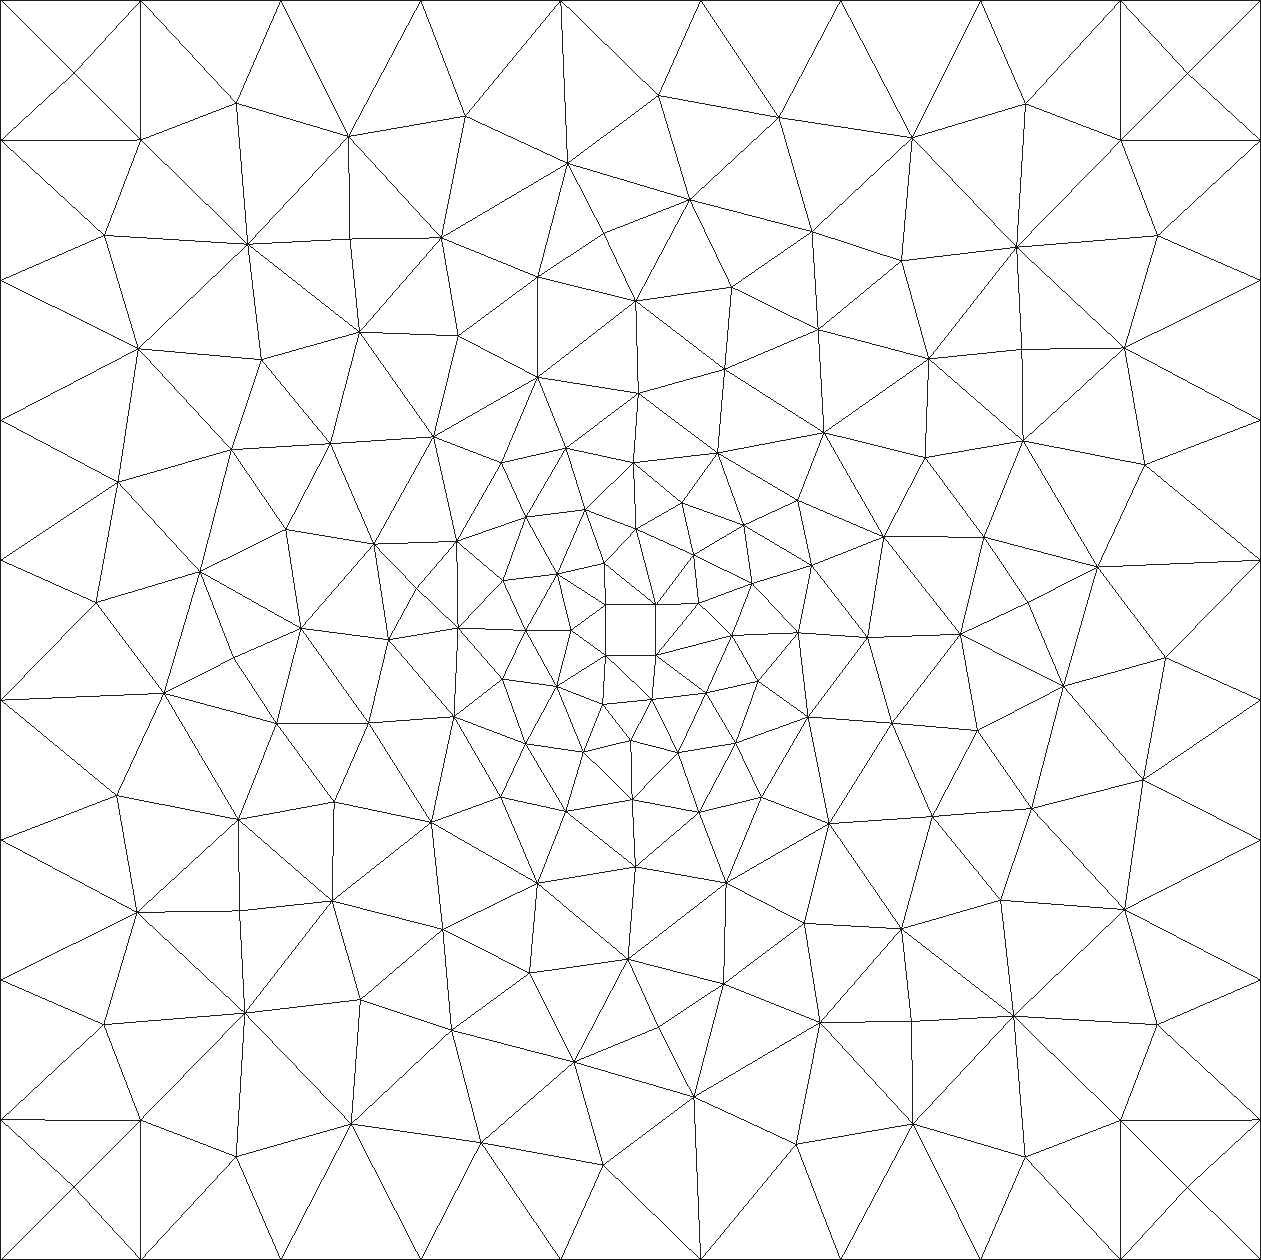
\includegraphics[scale=0.09]{Figures/AdaptiveADRkappa1E-1_mesh0.png}
            }
            \subcaptionbox{Primal solution at $t=10$.}{
                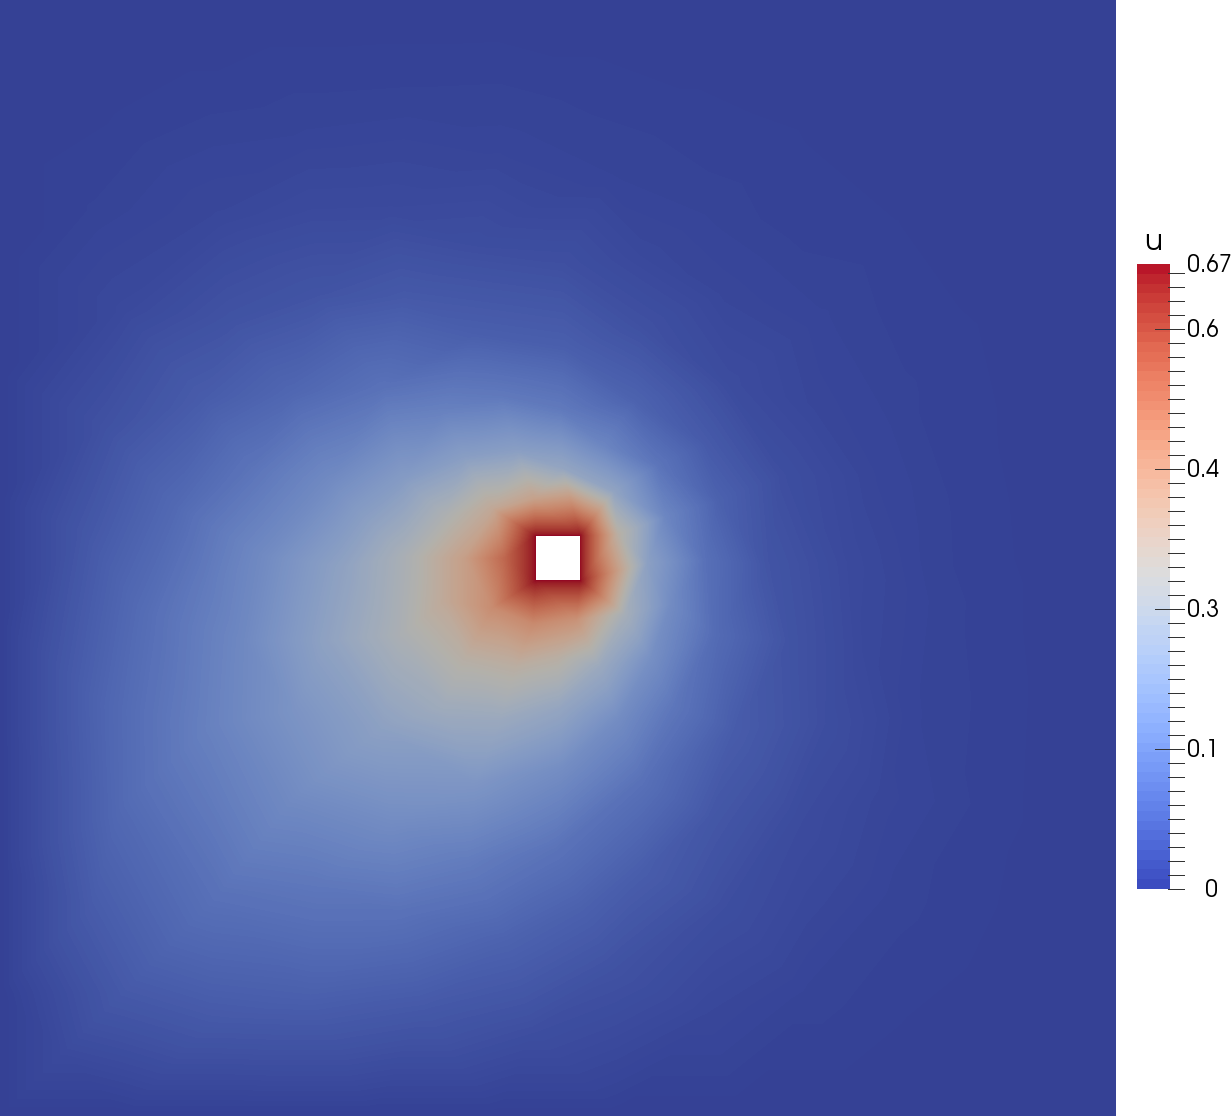
\includegraphics[scale=0.1]{Figures/AdaptiveADRkappa1E-1_u0.png}
            }
            \subcaptionbox{Error indicators}{
                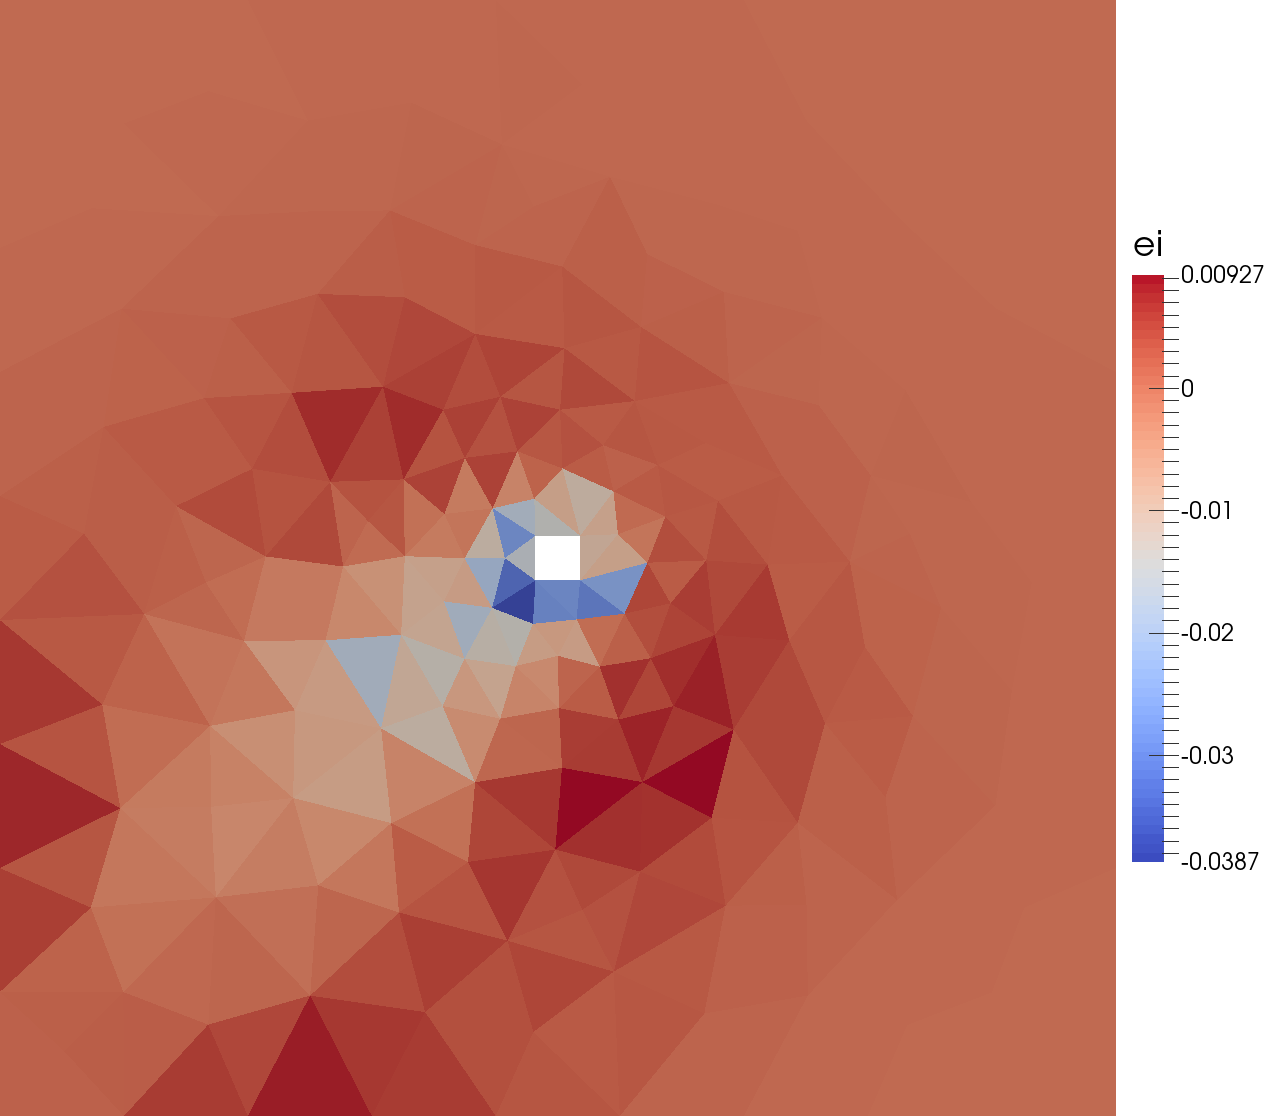
\includegraphics[scale=0.1]{Figures/AdaptiveADRkappa1E-1_ei0.png}
            }
            \subcaptionbox{Dual solution at $t=0$.}{
                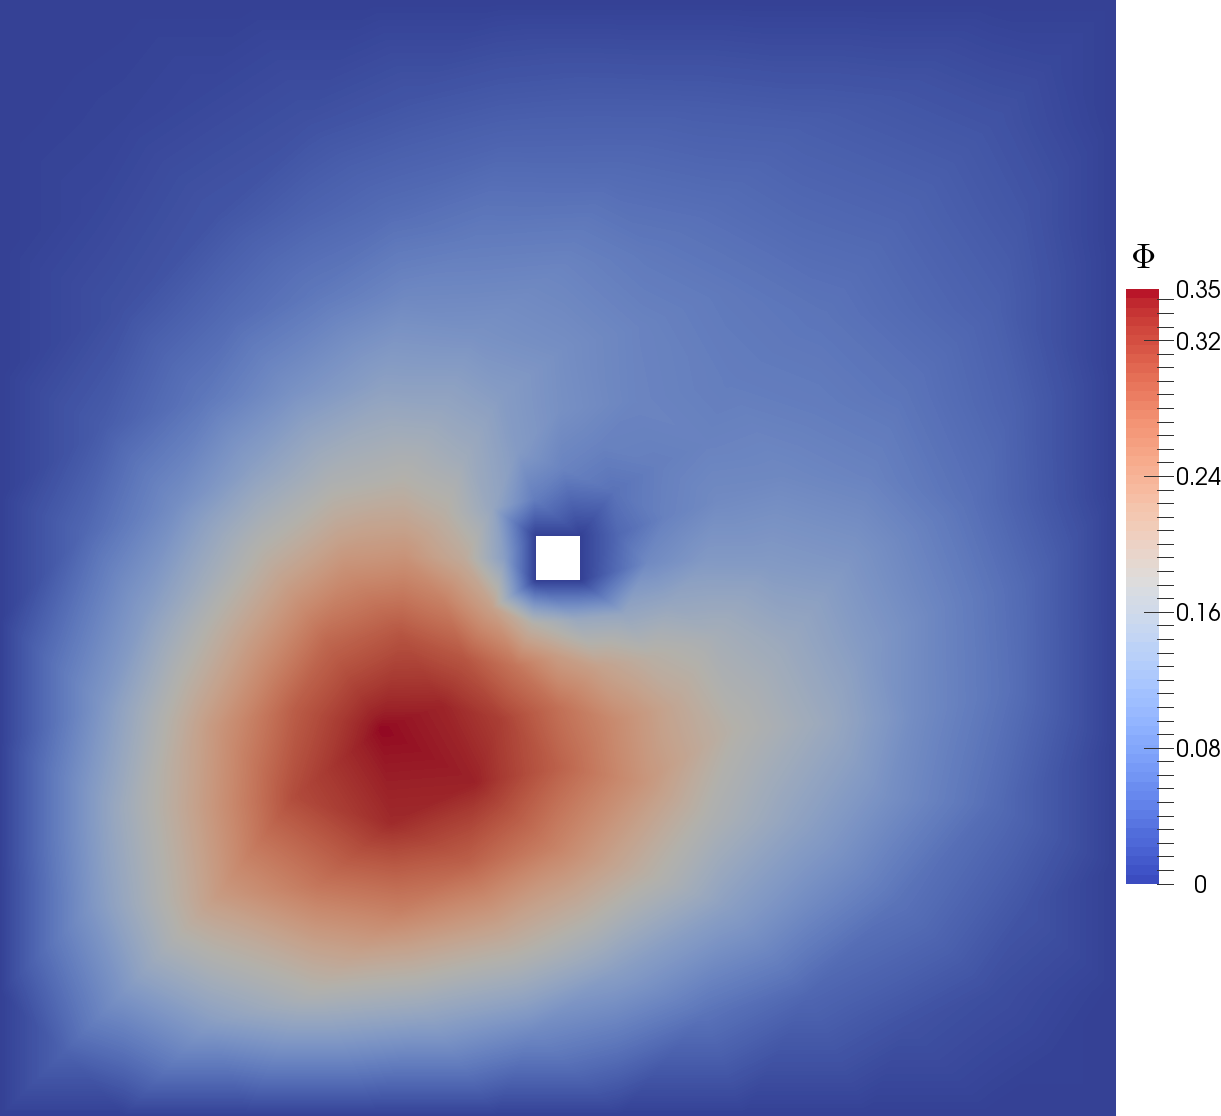
\includegraphics[scale=0.1]{Figures/AdaptiveADRkappa1E-1_uDual0.png}
            }
        \end{minipage}
        \begin{minipage}[t]{0.49\textwidth}
            \centering
            \subcaptionbox{$25^{th}$ adaptive mesh}{
                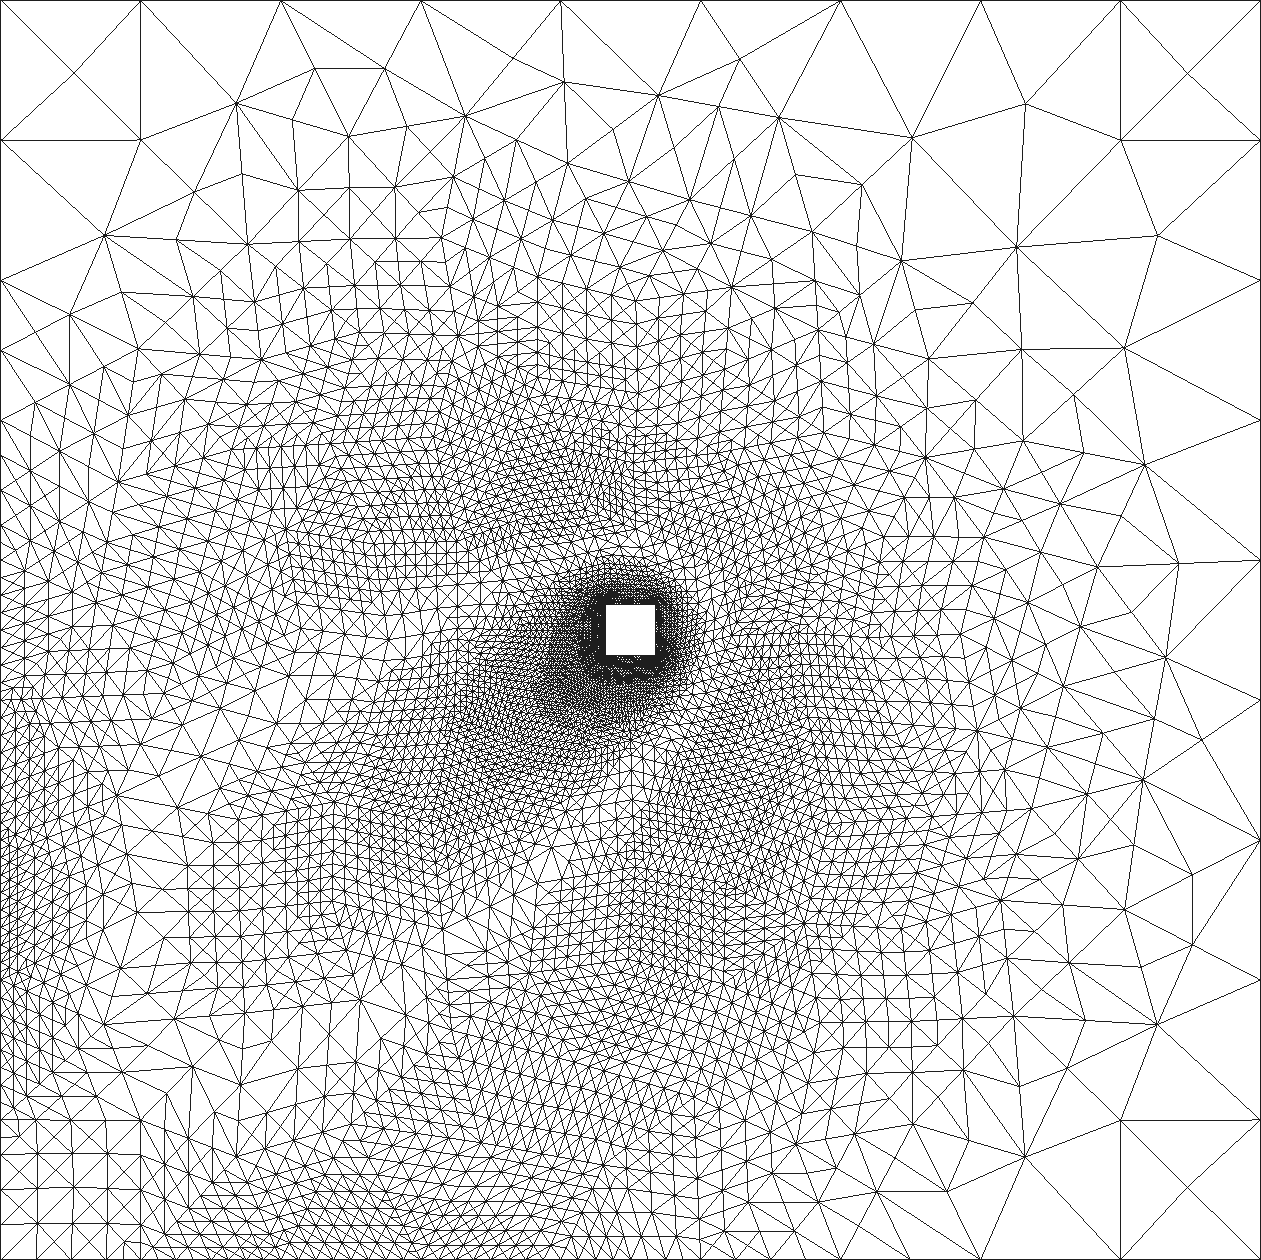
\includegraphics[scale=0.09]{Figures/AdaptiveADRkappa1E-1_mesh25.png}
            }
            \subcaptionbox{Primal solution at $t=10$.}{
                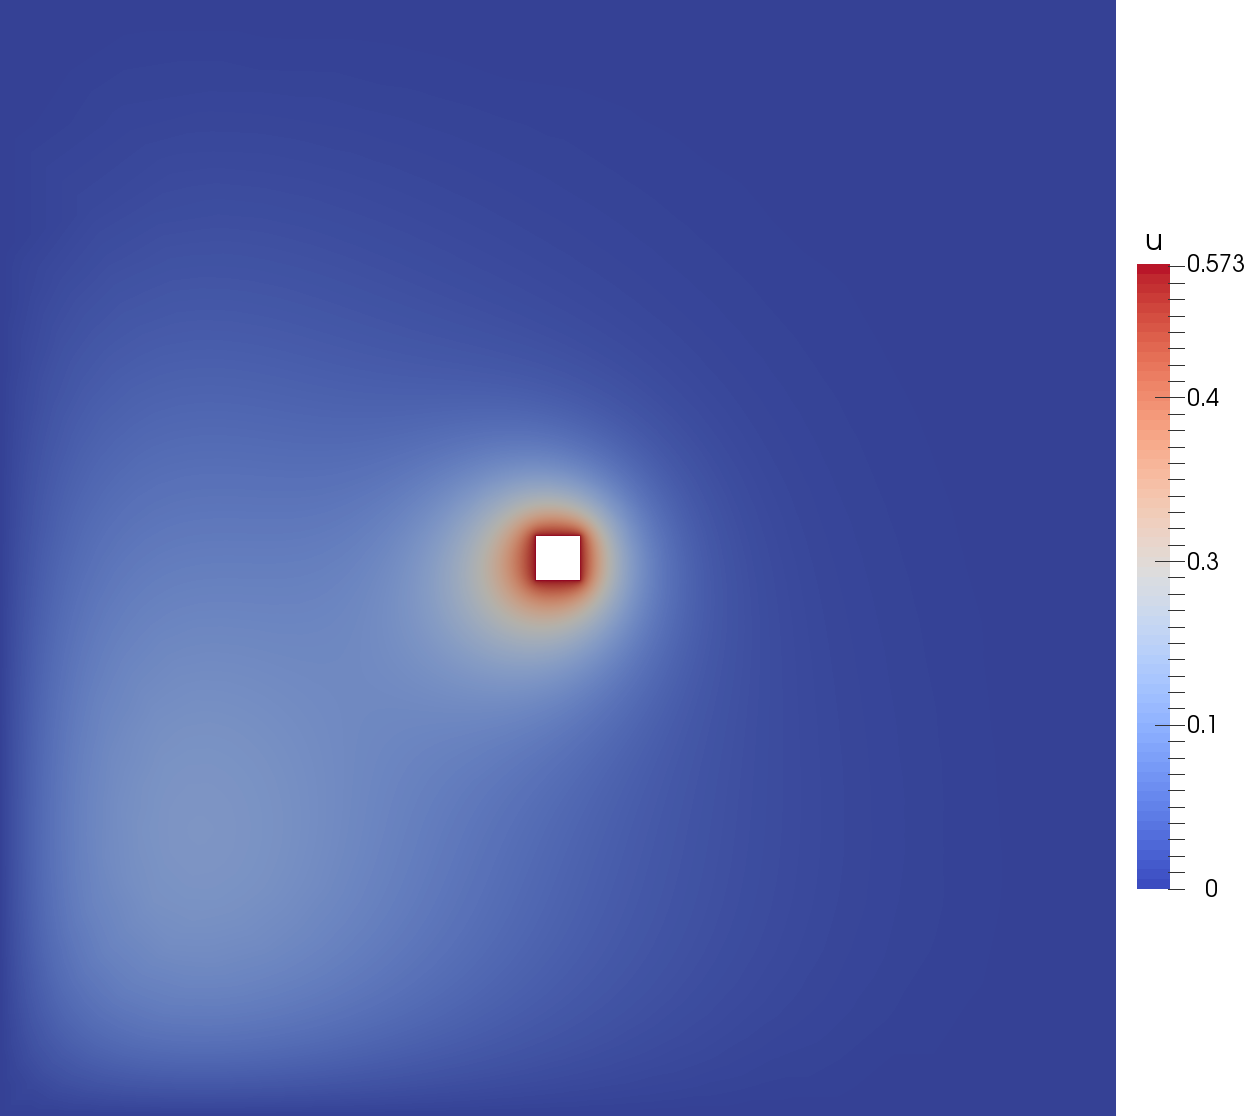
\includegraphics[scale=0.1]{Figures/AdaptiveADRkappa1E-1_u25.png}
            }
            \subcaptionbox{Error indicators}{
                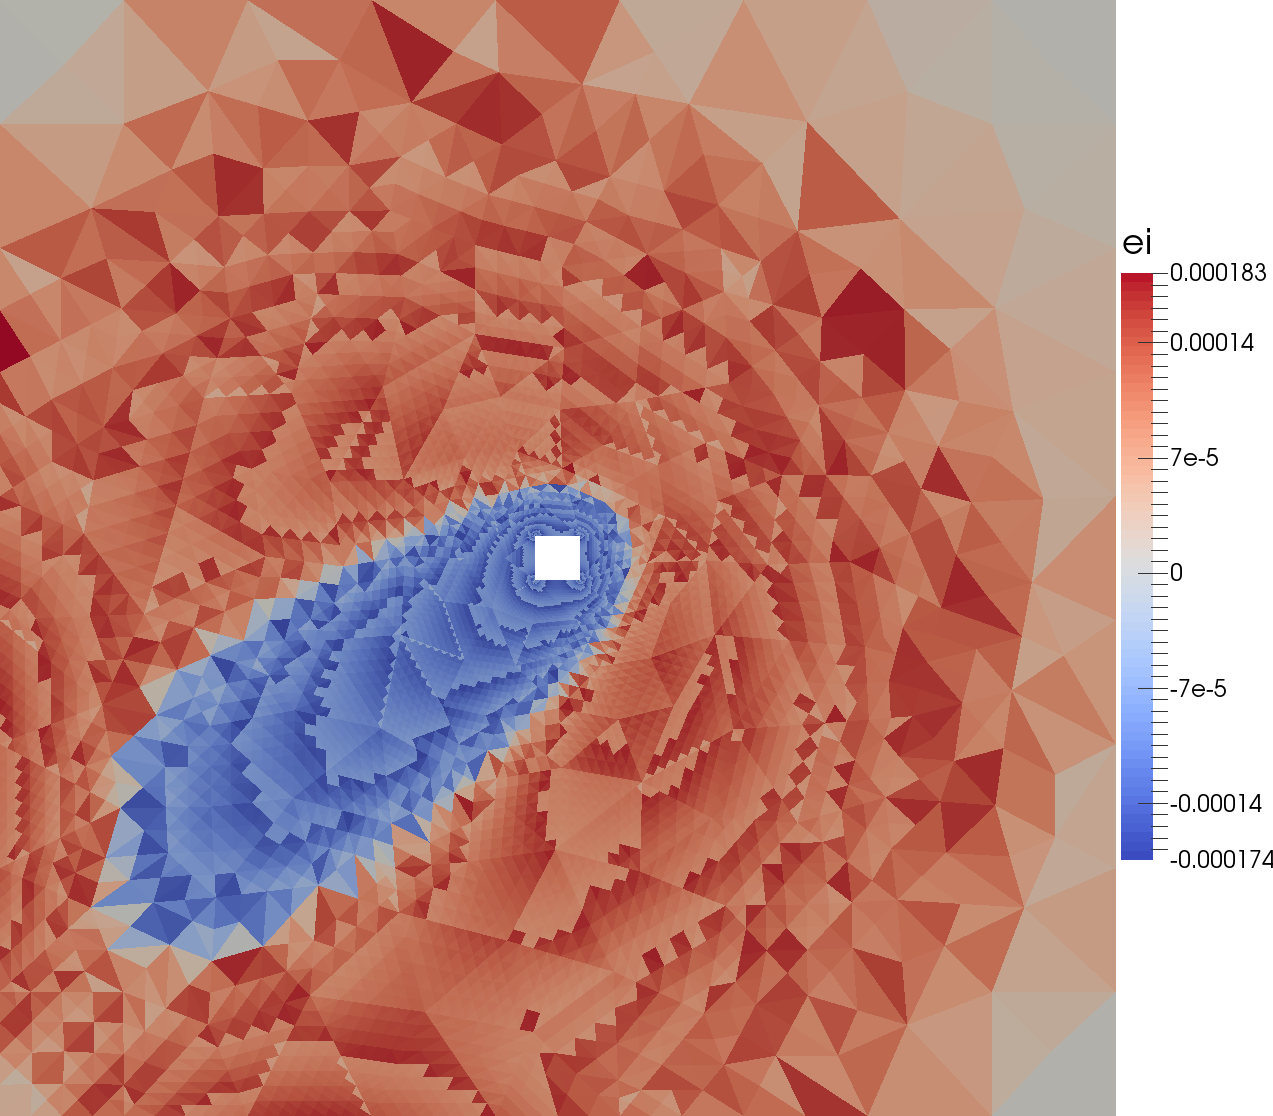
\includegraphics[scale=0.1]{Figures/AdaptiveADRkappa1E-1_ei25.png}
            }
            \subcaptionbox{Dual solution at $t=0$.}{
                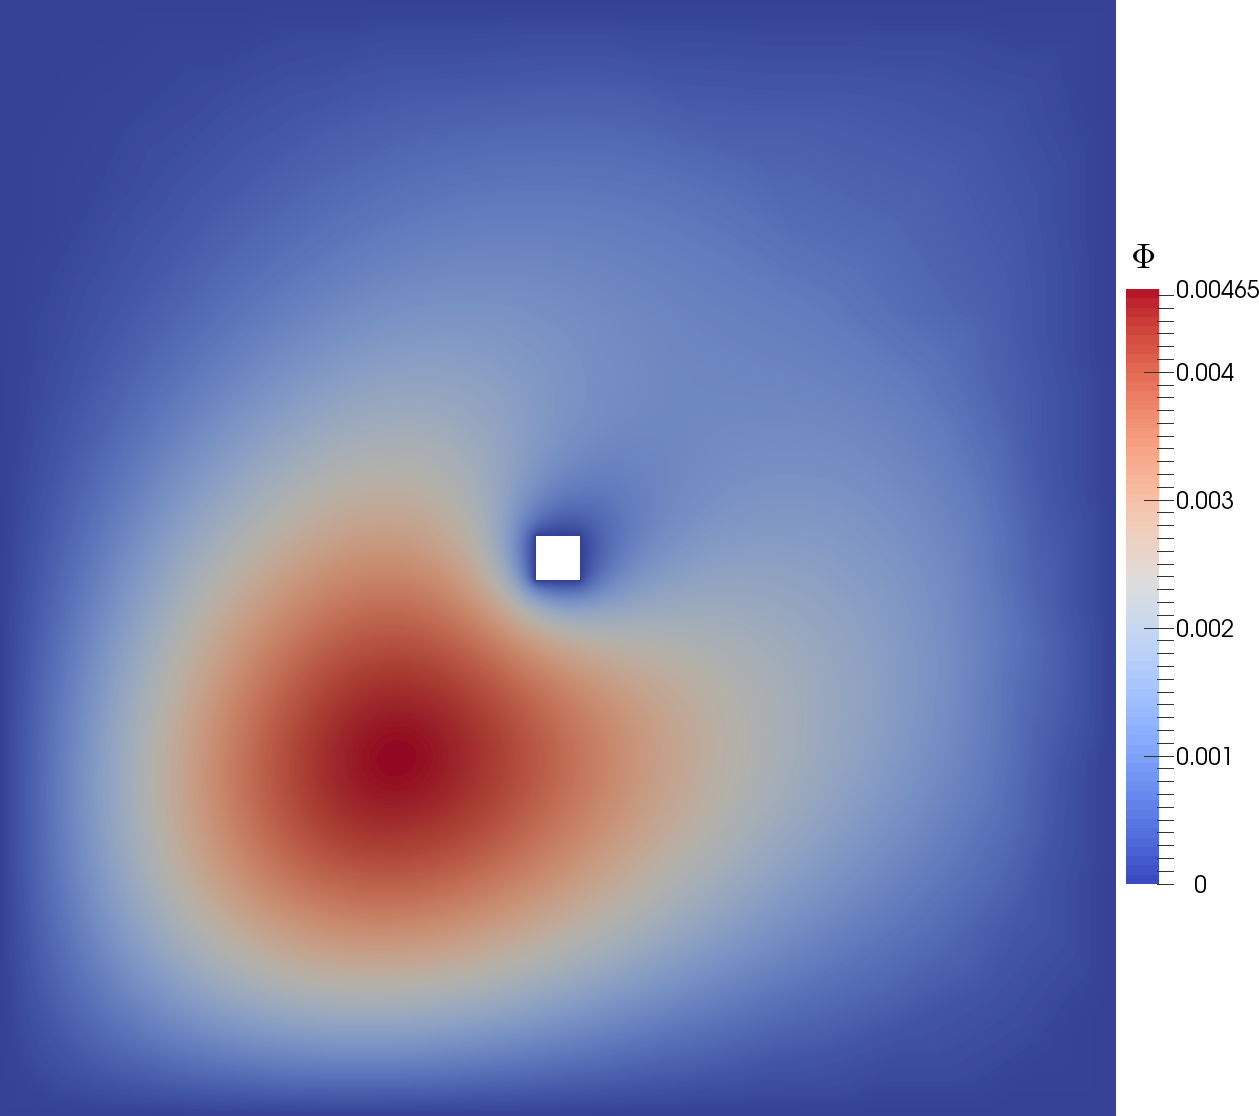
\includegraphics[scale=0.1]{Figures/AdaptiveADRkappa1E-1_uDual25.png}
            }
        \end{minipage}
        \caption{Comparison of the Initial Mesh (Left), $190$ DOFs, to the
                 $25^{th}$ Adaptive mesh (Right), $7\, 906$ DoFs, for ARD with
                 $\kappa=0.1$.}
    \end{figure}

    \begin{figure}[h]
        \centering
        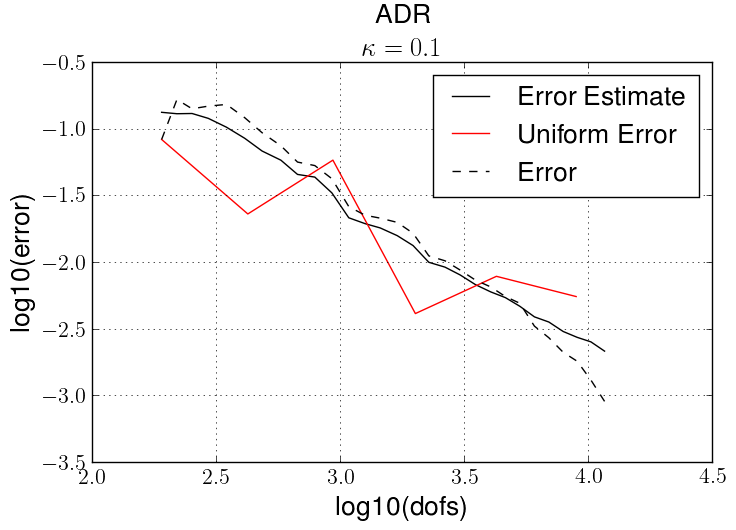
\includegraphics[scale=0.5]{Figures/AdaptiveADRkappa1E-1.png}
        \caption{Adaptive error estimate versus ``true'' error for the solution
            for the ARD equation with $\kappa=0.1$.}
        \label{fig:ADRk1E-1_err}
    \end{figure}
\end{test}

\begin{test}[Convection Dominated ARD, $\kappa = 1\times10^{-5}$] \label{tst:ADRk1E-5}
    In this test we simulate the ARD using convection dominated parameters, i.e.
    \begin{align*}
        \alpha &= 1, \\
        \kappa &= 1\time 10^{-5}, \\
        \beta &= \begin{bmatrix} -1 \\ -1.61 \end{bmatrix}.
    \end{align*}
    This will result in a concentration, $u$, which is more localized and thus
    the goal oriented adaptivity will perform much better compared to the
    uniform refinement.  As expected this can be observed when looking at the
    comparison of error for the goal oriented adapted and uniform adaptivity in
    \autoref{fig:ADRk1E-5_err}. Additionally, we observe that the solution on
    the initial mesh with $190$ DoFs does look overly dispersive, which is
    partly due to the GLS stabilization used, since it the dispersivity of the
    stabilizationi is dependent on the mesh size. Thus, the coarser mesh results
    in higher dispersion, where as the fine mesh solution, $25^{th}$ adapted
    mesh with $39\, 044$ DoFs, results in a small amount of diffusion added to
    the area in which the concentration is highest. In this case the diffusion
    added by the GLS stabilization acts to dampen the Gibs phenomenon resulting
    from the abrupt change in concentration. However, as can be seen there is a
    small amount of Gibs phenomenon still present, which is manifested in
    negative concentrations. The adaptive method does well in its refinement
    strategy, in that it refines mostly in the area where the Gibs phenomenon
    is occurring.

    We also note that the value of the BC at the inner square, $\Omega_2$, is
    $u = 5$ for the final time, $T=10$, and thus the initial mesh solution is
    clearly wrong.

    \begin{figure}[h]
        \centering
        \begin{minipage}[t]{0.49\textwidth}
            \centering
            \subcaptionbox{Initial mesh}{
                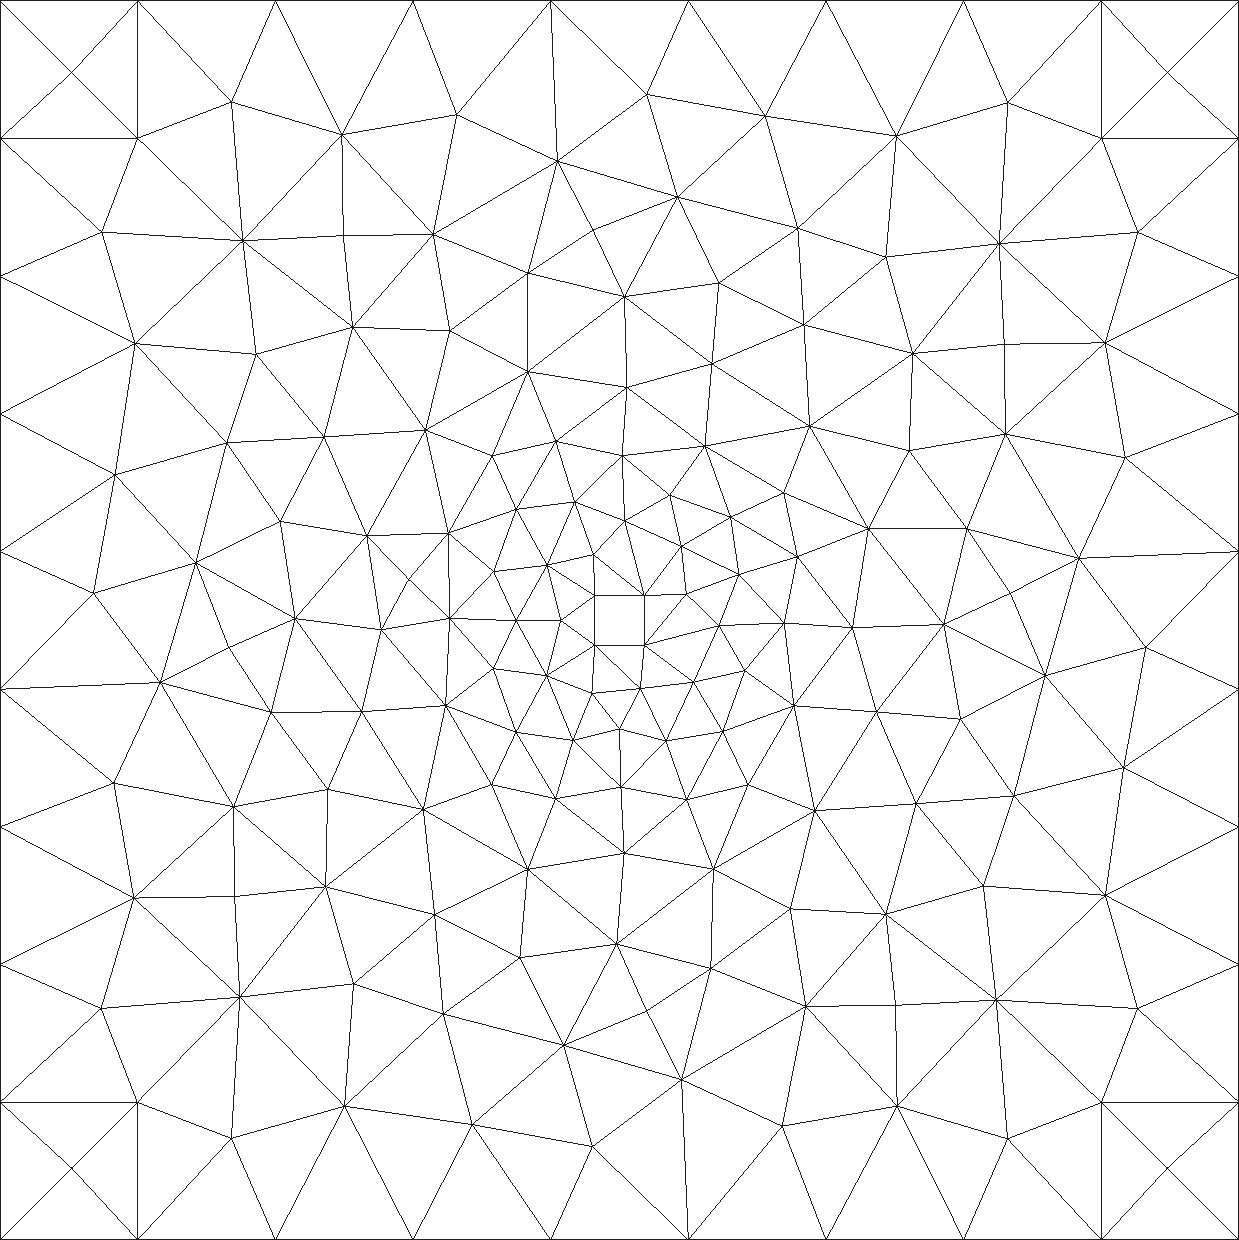
\includegraphics[scale=0.09]{Figures/AdaptiveADRkappa1E-5_mesh0.png}
            }
            \subcaptionbox{Primal solution at $t=10$.}{
                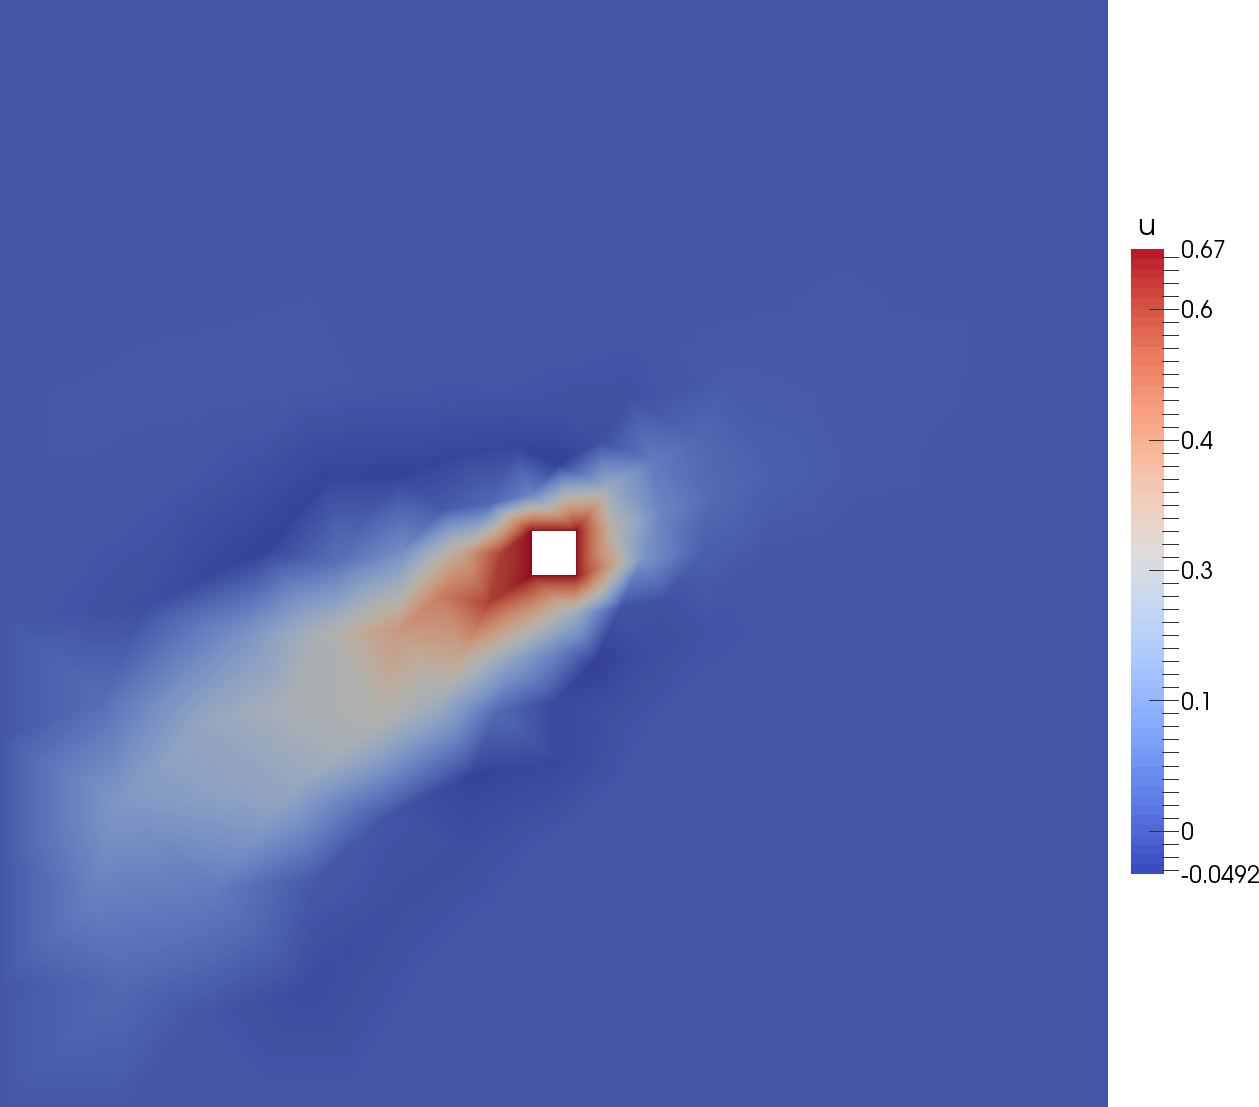
\includegraphics[scale=0.1]{Figures/AdaptiveADRkappa1E-5_u0.png}
            }
            \subcaptionbox{Error indicators}{
                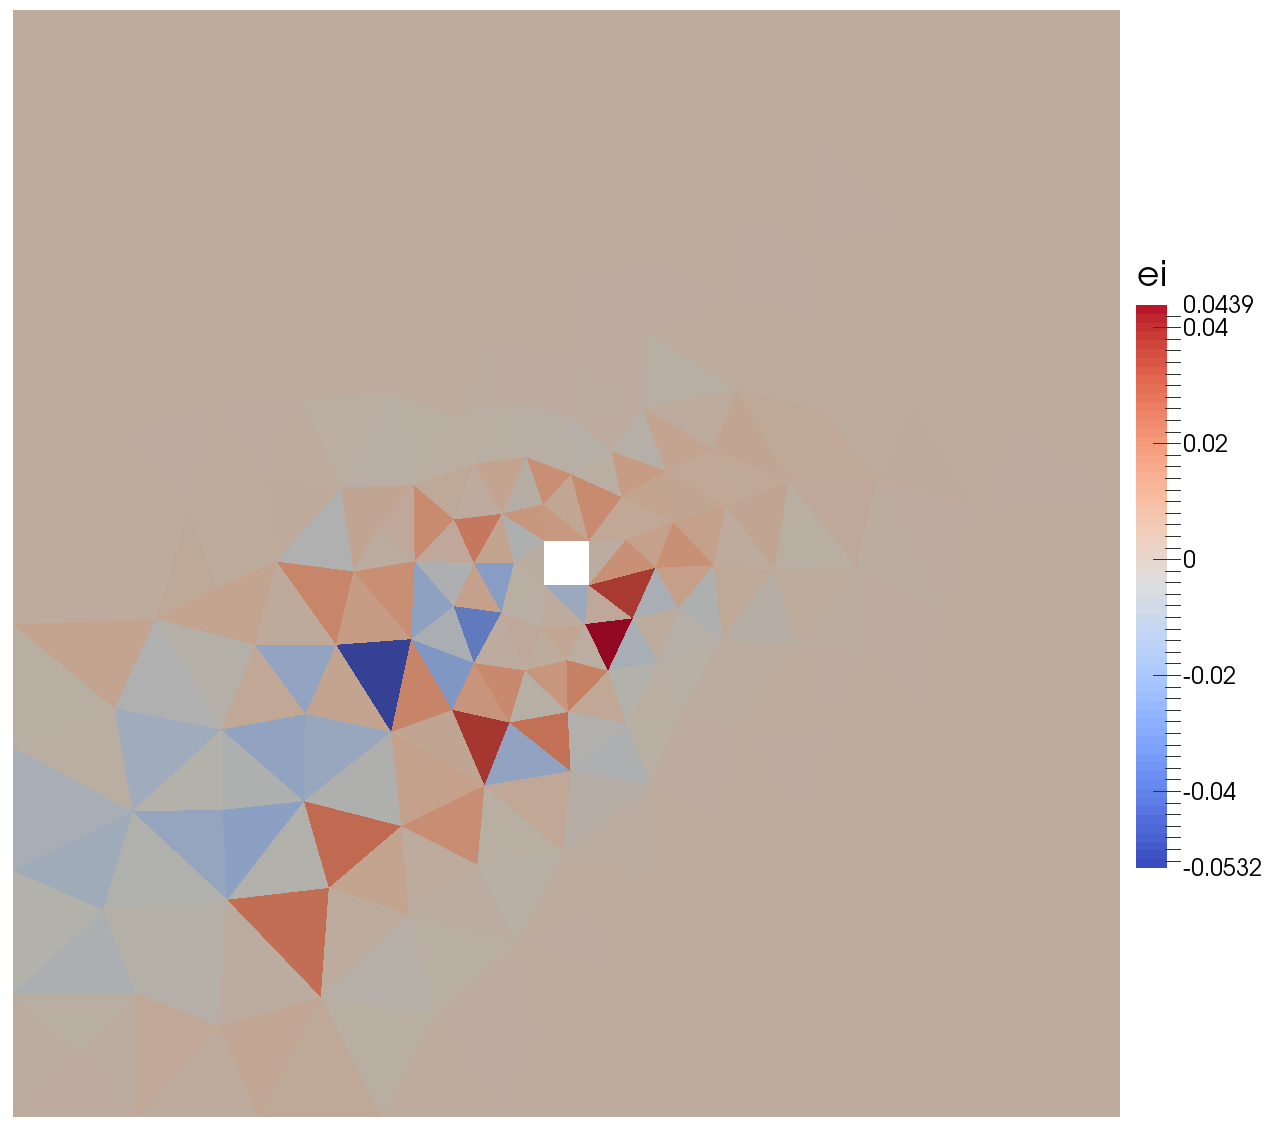
\includegraphics[scale=0.1]{Figures/AdaptiveADRkappa1E-5_ei0.png}
            }
            \subcaptionbox{Dual solution at $t=0$.}{
                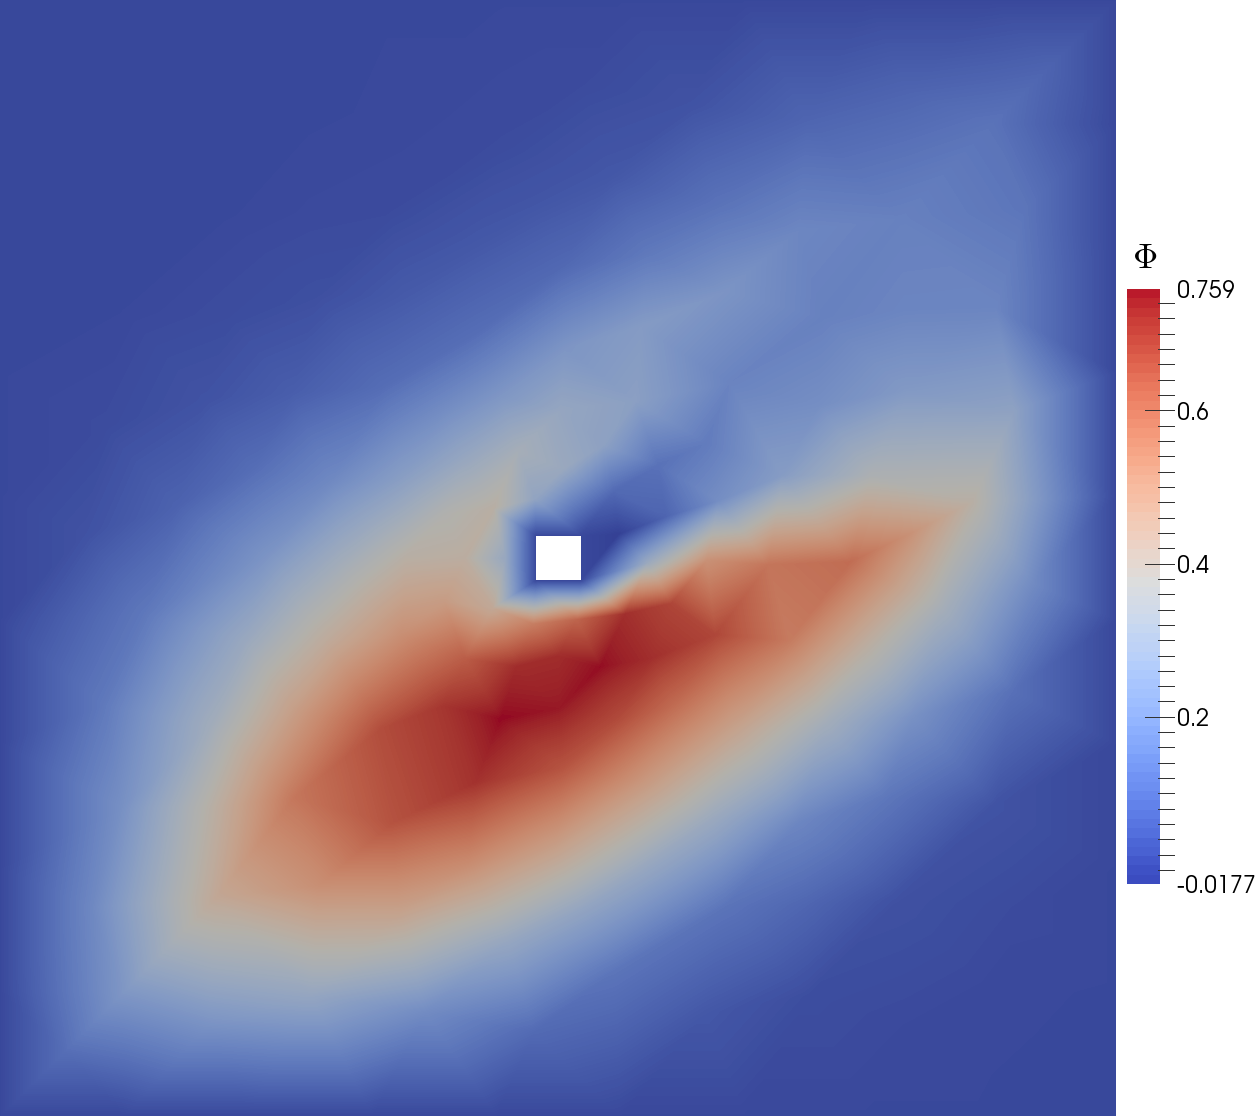
\includegraphics[scale=0.1]{Figures/AdaptiveADRkappa1E-5_uDual0.png}
            }
        \end{minipage}
        \begin{minipage}[t]{0.49\textwidth}
            \centering
            \subcaptionbox{$25^{th}$ adaptive mesh}{
                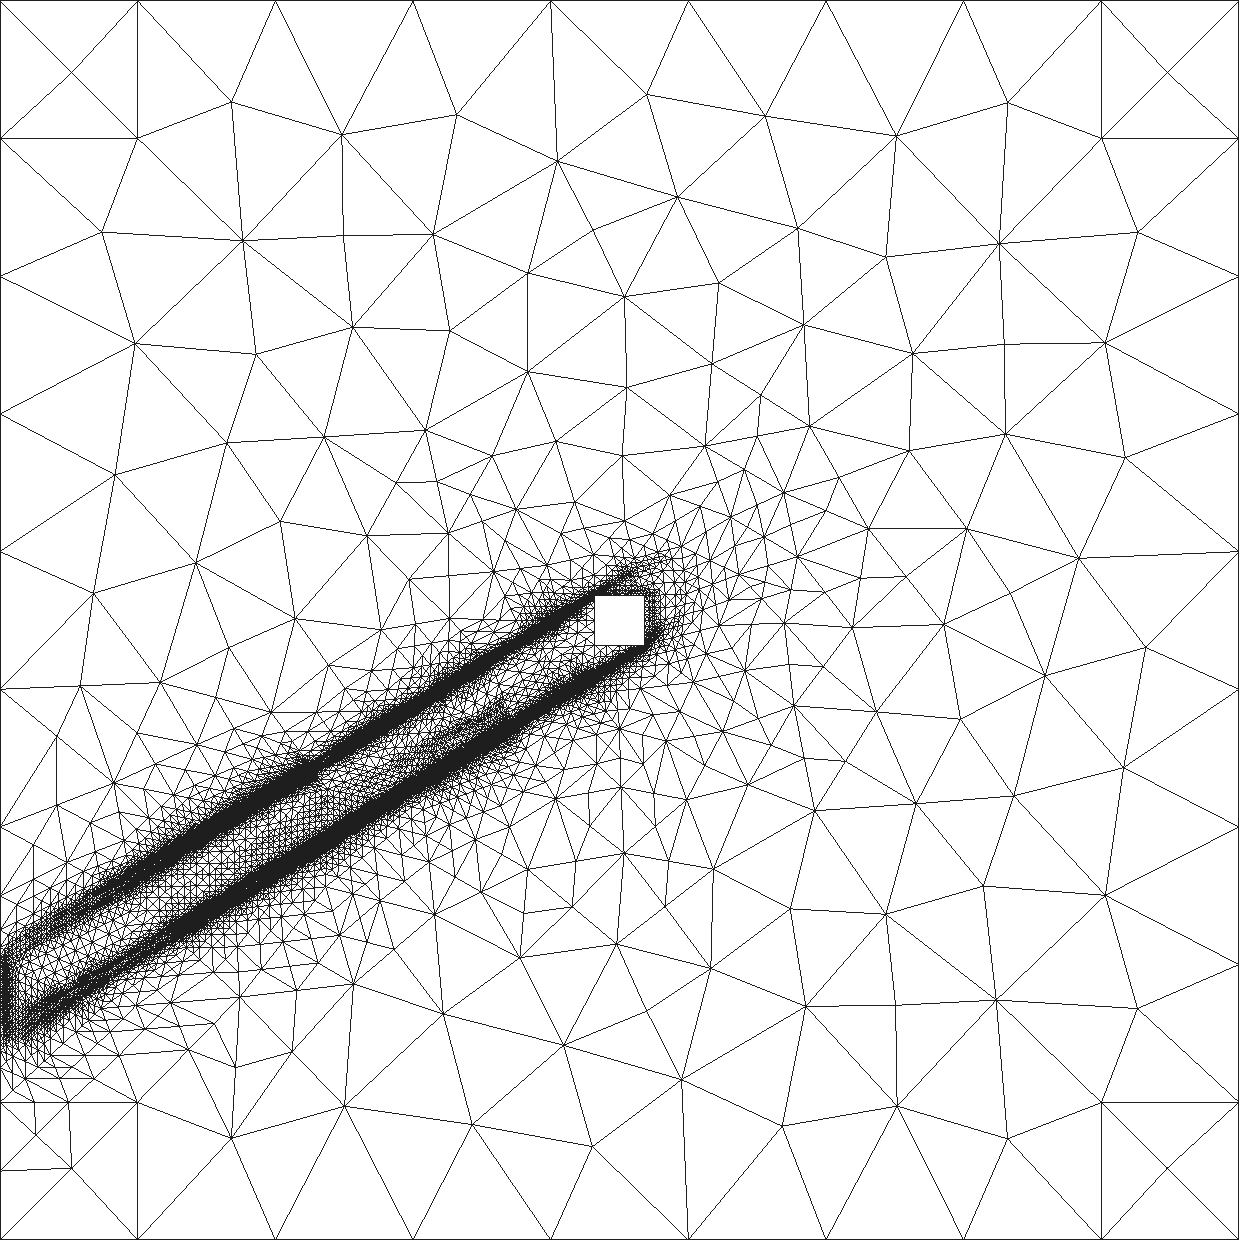
\includegraphics[scale=0.09]{Figures/AdaptiveADRkappa1E-5_mesh25.png}
            }
            \subcaptionbox{Primal solution at $t=10$.}{
                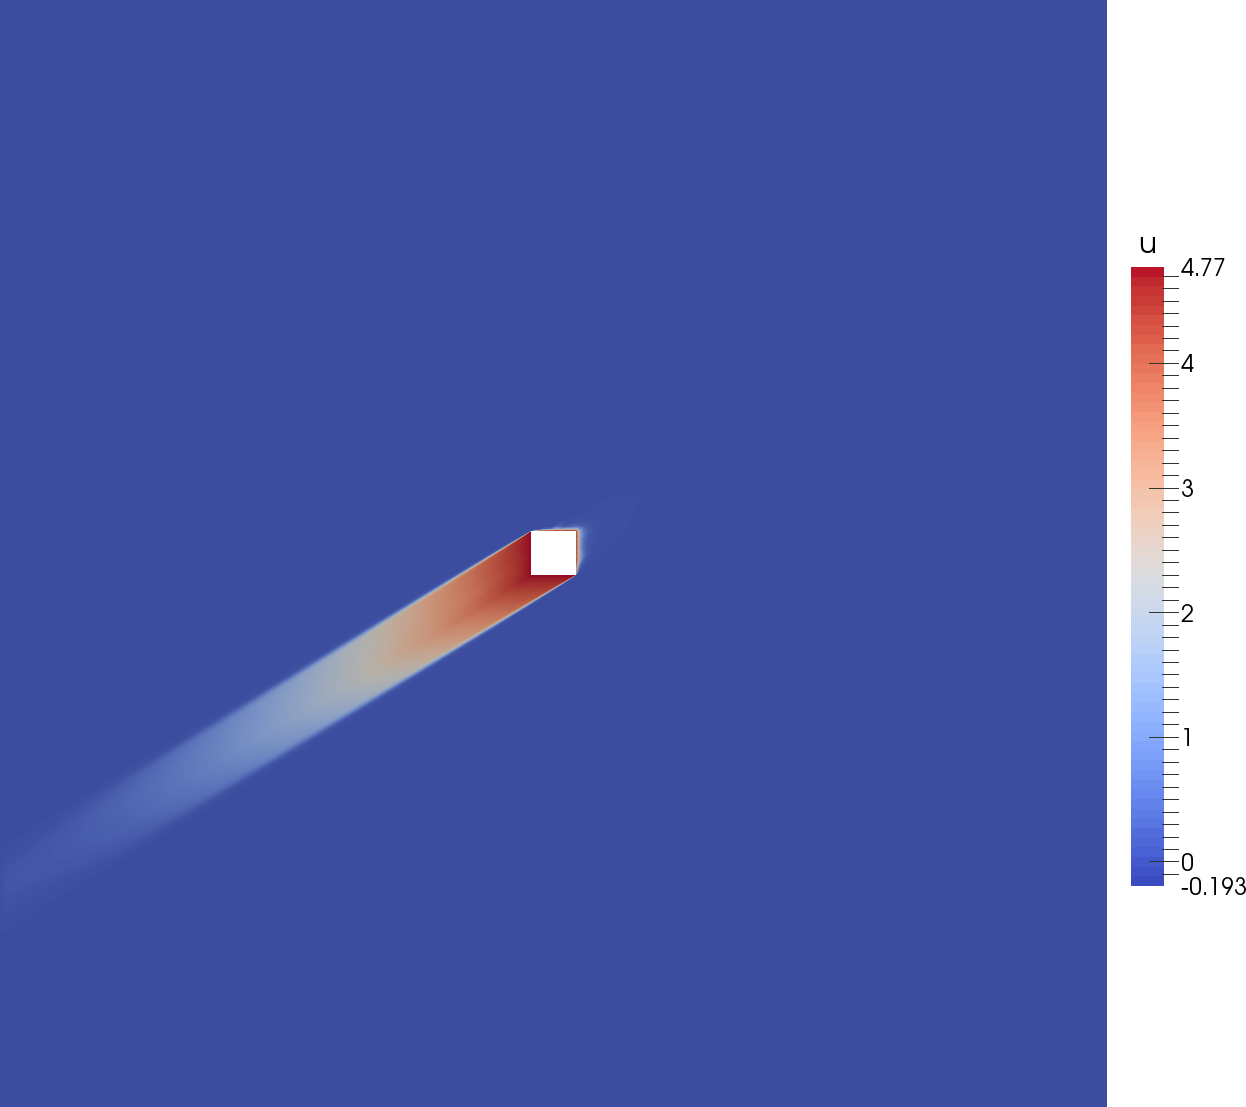
\includegraphics[scale=0.1]{Figures/AdaptiveADRkappa1E-5_u25.png}
            }
            \subcaptionbox{Error indicators}{
                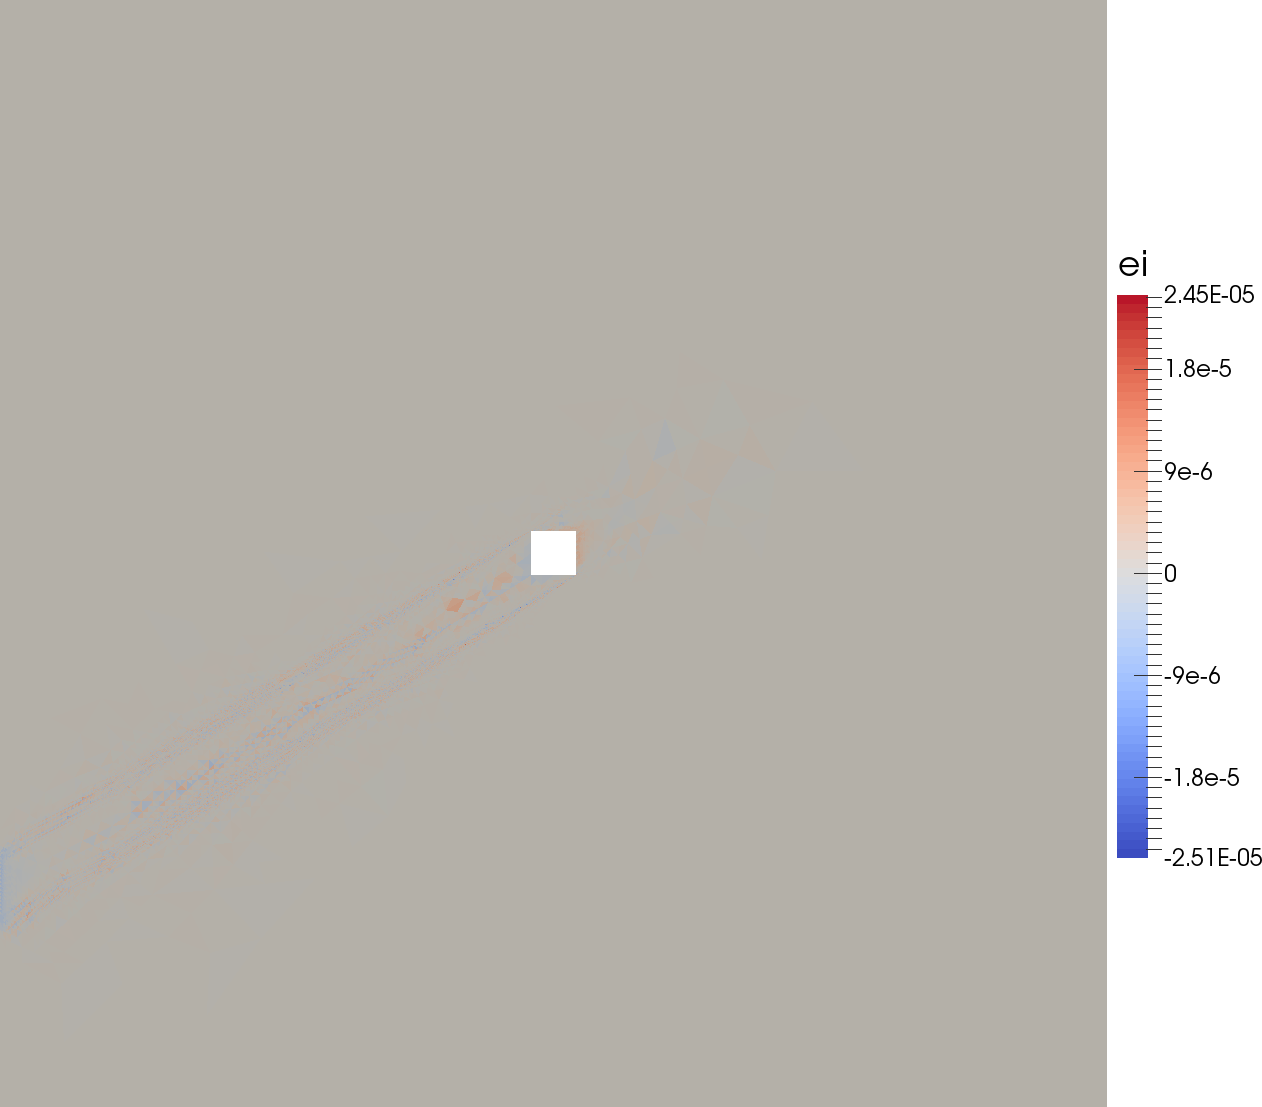
\includegraphics[scale=0.1]{Figures/AdaptiveADRkappa1E-5_ei25.png}
            }
            \subcaptionbox{Dual solution at $t=0$.}{
                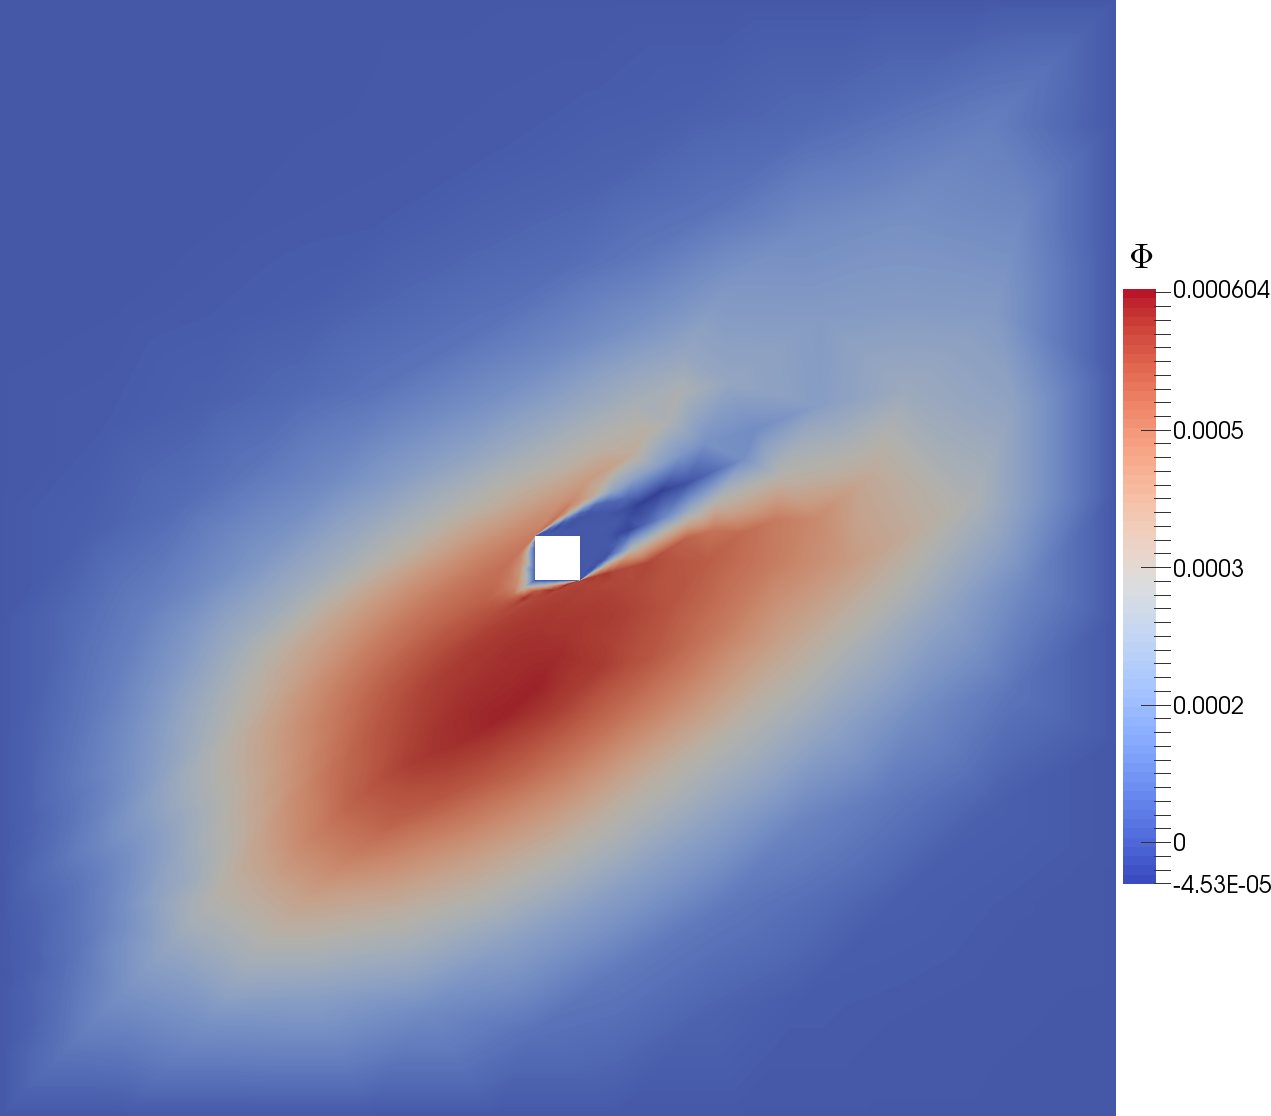
\includegraphics[scale=0.1]{Figures/AdaptiveADRkappa1E-5_uDual25.png}
            }
        \end{minipage}
        \caption{Comparison of the Initial Mesh (Left), $190$ DOFs, to the
                 $25^{th}$ Adaptive mesh (Right), $39\, 044$ DoFs, for ARD with
                 $\kappa=1\times 10^{-5}$.}
    \end{figure}

    \begin{figure}[h]
        \centering
        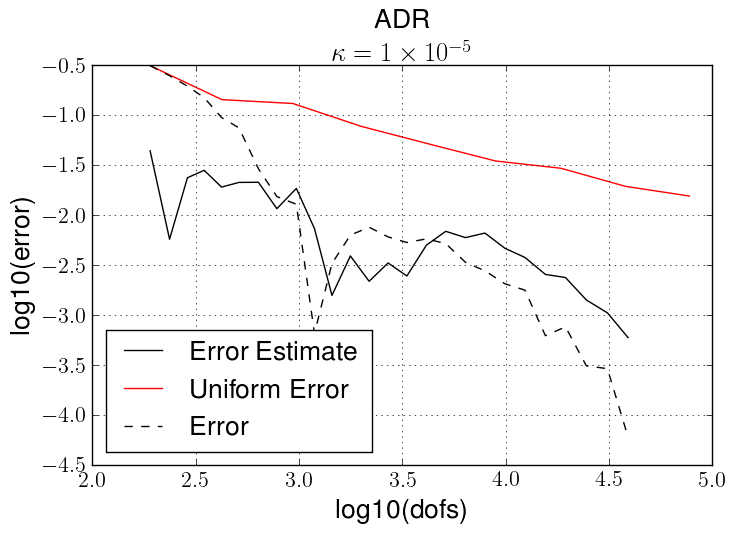
\includegraphics[scale=0.5]{Figures/AdaptiveADRkappa1E-5.png}
        \caption{Adaptive error estimate versus ``true'' error for the solution
            for the ARD equation with $\kappa=1\times 10^{-5}$.}
        \label{fig:ADRk1E-5_err}
    \end{figure}

\end{test}

\subsection{Non-Linear Problems}

\subsubsection{Navier-Stokes}

In this subsection we demonstrate the effectiveness of \autoref{alg:Adaptivity}
applied to problems where the with non-linear terms. In particular, we look at
applying \autoref{alg:Adaptivity} to the Incompressible Navier-Stokes and the
Variable Density Incompressible Navier-Stokes. In both cases, we solve each test
case using a Galerkin\slash~Least-Squares (GLS) stabilized $cG(1)cG(1)$finite
element, where the first cG(1) indicates that the test and trial functions are
both piecewise linear, while the second cG(1) indicates that the test piecewise
constants and the trial functions are continuous piecewise linear.

For the test problems \ref{tst:Drag} and \ref{tst:Velocity} we are concerned
with the Incompressible Navier-Stokes with constant kinematic viscosity,
$\nu>0$, in a domain $\Omega\subset \R^d$, with boundary $\partial \Omega$, i.e.
where the strong residual is given by
\begin{equation}
    \begin{split}
      \mathbf{u}_t + \left( \mathbf{u} \cdot \nabla \right) \mathbf{u} - \nu\,
          \Delta \mathbf{u} + \nabla p = \mathbf{f}, \quad \mathbf{x} \in \Omega \\
          \nabla \cdot \mathbf{u} = 0, \quad \mathbf{x} \in \Omega
    \end{split}
  \label{eqn:NSE}
\end{equation}
Given a step size $k$ and applying the $cG(1)cG(1)$finite element discretization
to \autoref{eqn:NSE} with $V = (v, q) \in X \subset [H^1_0(\Omega)]^d \times
H^1(\Omega)$ gives the following weak residual
\begin{equation}
  \begin{split}
    r(\bar{U}^n; V) &= \left(\mathbf{u}^n - \mathbf{u}^{n-1}, v\right)\,k^{-1}
        + (\left( \bar{\mathbf{u}}^n \cdot \nabla \right) \bar{\mathbf{u}}^n, v) \\
        &\quad+ \nu\, (\nabla \bar{\mathbf{u}}^n, \nabla v)
        + (\nabla p^n, v) - (\mathbf{f}, v)
        + (\nabla \cdot \bar{\mathbf{u}}^n, v) = 0
  \end{split}
  \label{eqn:WeakNSE}
\end{equation}
where $\bar{U}^n = (\bar{\mathbf{u}}^n,p)$, and $\bar{\mathbf{u}}^n =
\frac{1}{2}\left(\mathbf{u}^n + \mathbf{u}^{n-1}\right)$. Given the solution
$U=(\mathbf{u},p)$, since the elements we are concerned with (cG(1)cG(1)) have
test functions which are linear in space and constant in time the strong
residual is given by
\begin{equation}
    R(\bar{U}^n,U) = \begin{cases}
      \left(\mathbf{u} \cdot \nabla \right) \bar{\mathbf{u}}^n
        + \nabla p^n - \mathbf{f} = 0 \\
      \nabla \cdot \bar{\mathbf{u}}^n = 0.
    \end{cases}
  \label{eqn:StrongNSE}
\end{equation}
Finally, the GLS-cG(1)cG(1) discretization of \eqref{eqn:NSE} is given by
\begin{equation}
  r(\bar{U}^n,V) + SD_{\delta}^n(\bar{U}^n,V) = 0, \quad \forall V=(v,q) \in X.
  \label{eqn:G2}
\end{equation}
Here $SD_{\delta}^n$ is the GLS stabilization and is given by
\begin{equation}
  SD_{\delta}^n \equiv
    \delta_1 (\left(\bar{\mathbf{u}}^n \cdot \nabla \right) \bar{\mathbf{u}}^n
        + \nabla p^n - \mathbf{f},
      \left(\bar{\mathbf{u}}^n \cdot \nabla \right) v + \nabla q)
      + \delta_2 (\nabla \cdot \bar{\mathbf{U}}^n, \nabla \cdot v),
  \label{eqn:NSEStabilization}
\end{equation}
where $\delta_1 = \kappa_1 (k^{-1} + |\mathbf{u}^{n-1}|^2\, h^{-2})^{-1/2}$, and
$\delta_2 = \kappa_2 h$, while $\kappa_1$ and $\kappa_2$ are problem independent
constants of unit size. For each test case below we take the time-step to be
\begin{equation*}
  k = CFL\, \frac{\min_{\mathcal{T}_K}(h)}{|U_m|},
\end{equation*}
where $CFL=100$.

This following test cases are based on a benchmark problem from Sch\"afer and
Turek \cite[Test case 2D-2]{Schaefer1996}. Thus, we define the domain to be a
rectangular domain with a circle removed (see \autoref{fig:2DCylinder}). For the
inlet boundary condition we take
\begin{equation}
    u(0,y,t) = (4\, U_m\,y\, (H - y)/H^2, 0),
    \label{eqn:2DInlet}
\end{equation}
where $U_m = 1.5\, \text{m/s}$, $H = 0.41\, \text{m}$. For the kinematic
viscosity we take $\nu = 10^{-3}\, \text{m}^2\text{/s}$, resulting in a
Reynolds number of $Re=100$.

\begin{figure}[h]
    \centering
    \tikzstyle{next}=[->, thick, shorten <=1pt, shorten >=1pt]
    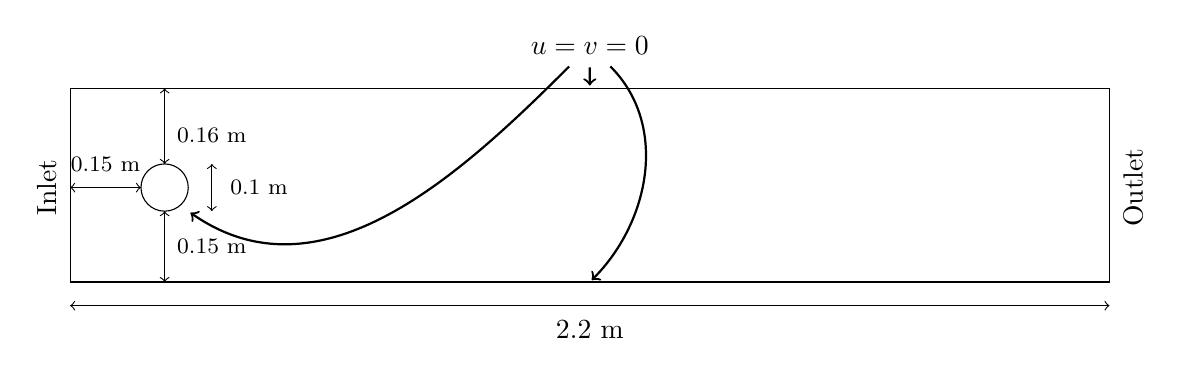
\begin{tikzpicture}[scale=6]
        \draw (0,0) -- (2.2,0) -- (2.2,0.41) -- (0,0.41) -- cycle;
        \draw (0.2,0.2) circle (0.05);
        \draw[<->] (0,-0.05) -- (2.2,-0.05);
        \draw (1.1,-0.1) node {2.2 m};
        \draw[<->] (0,0.2) -- (0.15,0.2);
        \draw (0.075,0.25) node {\footnotesize 0.15 m};
        \draw[<->] (0.2,0) -- (0.2,0.15);
        \draw (0.3,0.075) node {\footnotesize 0.15 m};
        \draw[<->] (0.2,0.25) -- (0.2,0.41);
        \draw (0.3,0.31) node {\footnotesize 0.16 m};
        \draw[<->] (0.3,0.15) -- (0.3,0.25);
        \draw (0.4,0.2) node {\footnotesize 0.1 m};
        \node[rotate=90] (outflow) at (2.25, 0.2) {Outlet};
        \node[rotate=90] (inflow) at (-0.05, 0.2) {Inlet};
        \node (NoFlow) at (1.1,0.5) {$u=v=0$};
        \draw[next] (NoFlow) to (1.1,0.41);
        \draw[next] (NoFlow) to [out=-45,in=45] (1.1,0);
        \draw[next] (NoFlow) to [out=-135,in=-35] (0.25,0.15);
    \end{tikzpicture}
    \caption{Geometry for \autoref{tst:Drag} and \autoref{tst:Velocity}}
    \label{fig:2DCylinder}
\end{figure}

\begin{test}[NSE, Drag Functional] \label{tst:Drag}
    \begin{equation}
        M(\bar{U}^n) := \int_I\! C_D\, dt,
        \label{eq:DragFunctional}
    \end{equation}
    where
    \begin{equation*}
        C_D = \frac{2}{\bar{u}^2\, D}F_D,
    \end{equation*}
    and
    \begin{equation*}
        \begin{bmatrix} F_D \\ F_L \end{bmatrix} =
            \int_{\partial \Omega_1}\! (p\, \mathbf{I} - \nu \nabla
                \mathbf{u})\cdot \mathbf{n}\, ds.
    \end{equation*}

    \begin{figure}[h]
        \centering
        \begin{minipage}[t]{0.49\textwidth}
            \centering
            \subcaptionbox{Initial mesh}{
                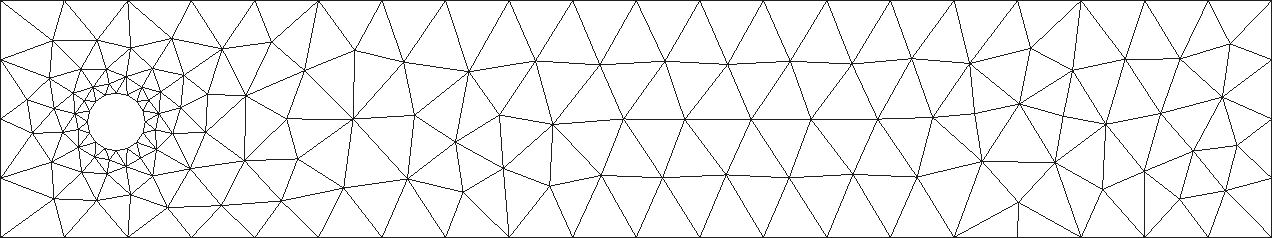
\includegraphics[scale=0.15]{Figures/AdaptiveNSEDragRe100_mesh0.png}
            }
            \subcaptionbox{Primal solution at $t=10$.}{
                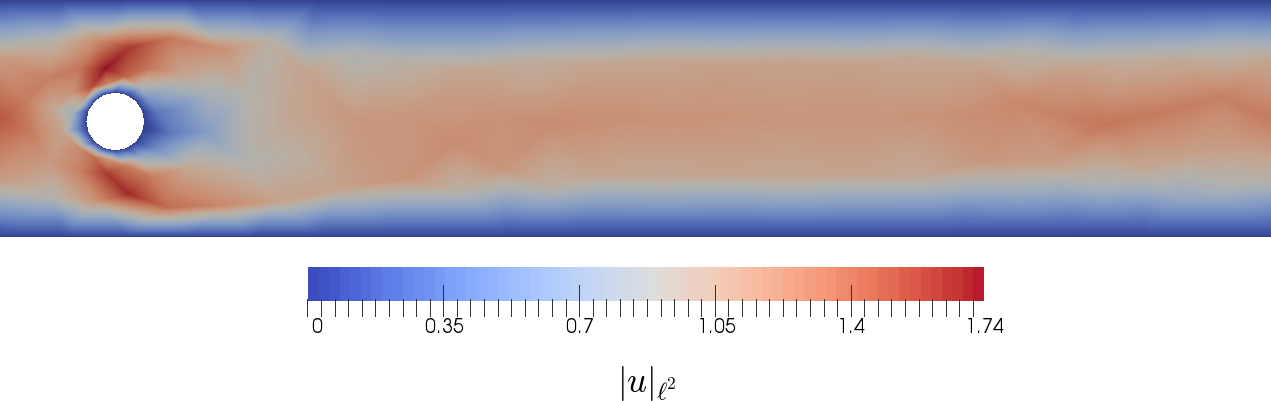
\includegraphics[scale=0.15]{Figures/AdaptiveNSEDragRe100_u0.png}
            }
            \subcaptionbox{Error indicators}{
                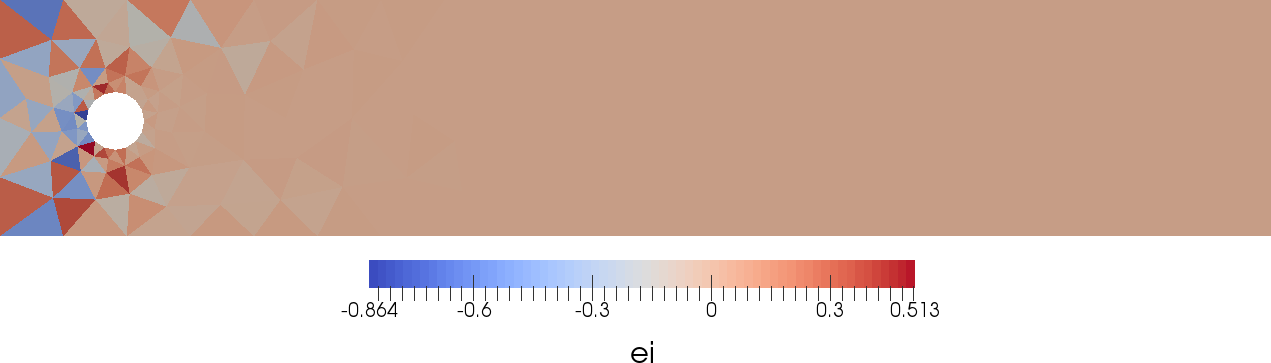
\includegraphics[scale=0.15]{Figures/AdaptiveNSEDragRe100_ei0.png}
            }
            \subcaptionbox{Dual solution at $t=0$.}{
                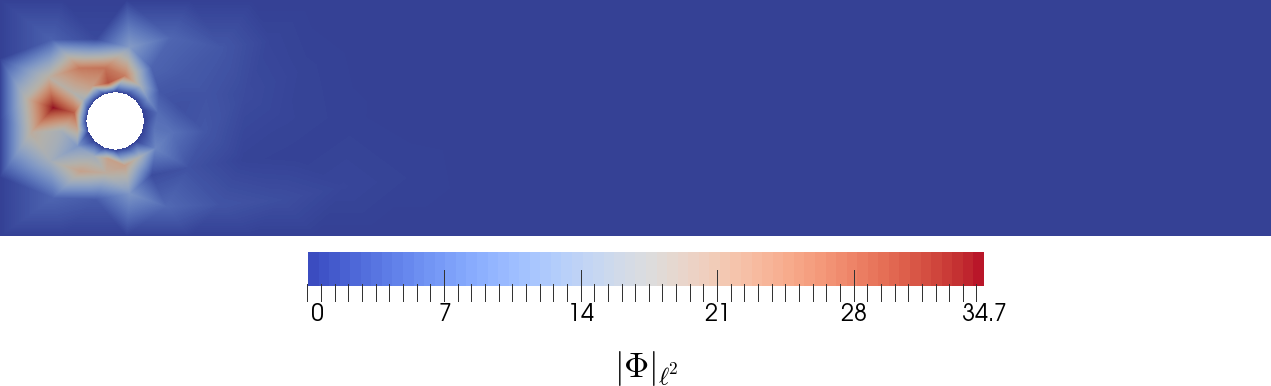
\includegraphics[scale=0.15]{Figures/AdaptiveNSEDragRe100_uDual0.png}
            }
        \end{minipage}
        \begin{minipage}[t]{0.49\textwidth}
            \centering
            \subcaptionbox{$25^{th}$ adaptive mesh}{
                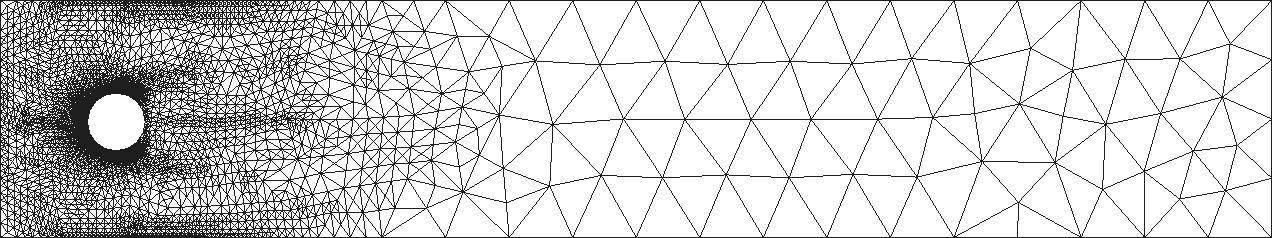
\includegraphics[scale=0.15]{Figures/AdaptiveNSEDragRe100_mesh25.png}
            }
            \subcaptionbox{Primal solution at $t=10$.}{
                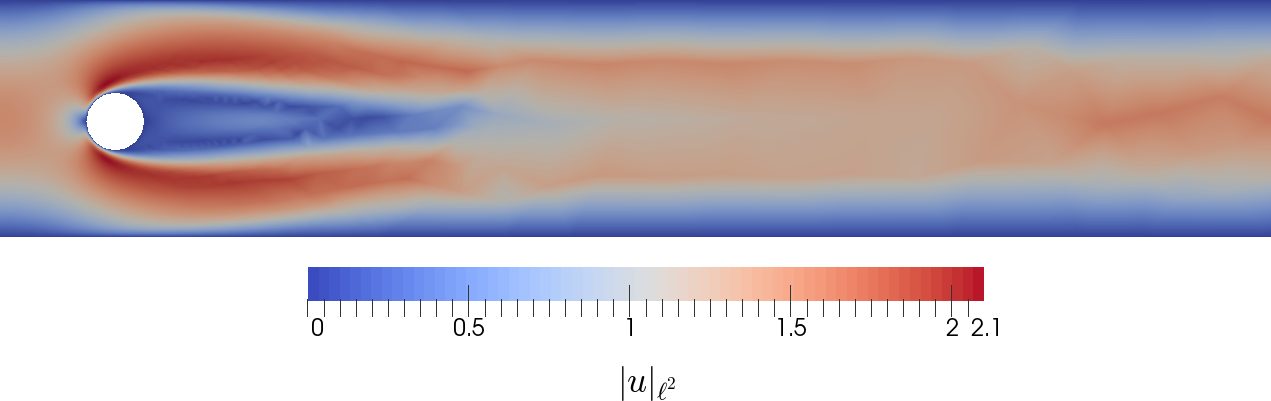
\includegraphics[scale=0.15]{Figures/AdaptiveNSEDragRe100_u25.png}
            }
            \subcaptionbox{Error indicators}{
                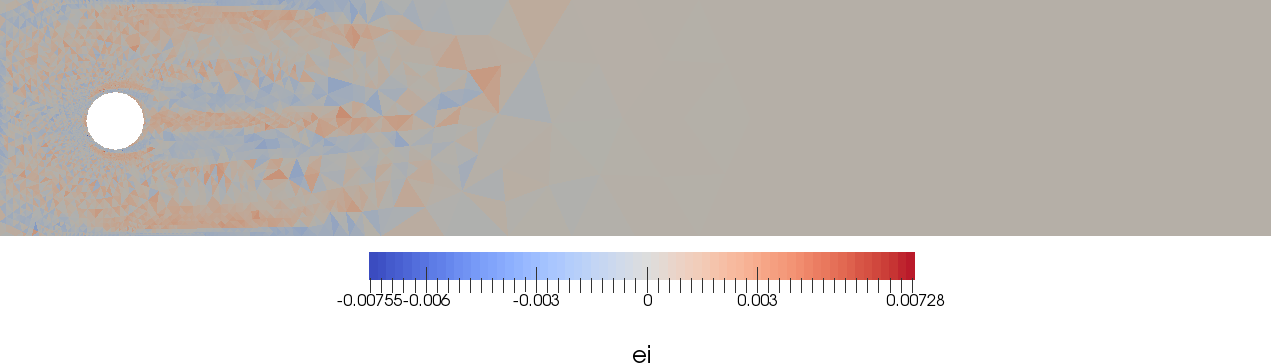
\includegraphics[scale=0.15]{Figures/AdaptiveNSEDragRe100_ei25.png}
            }
            \subcaptionbox{Dual solution at $t=0$.}{
                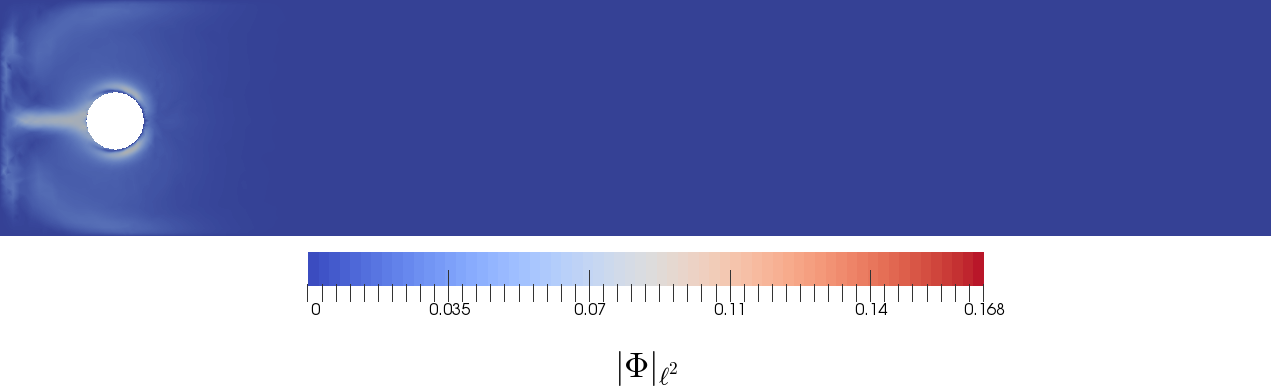
\includegraphics[scale=0.15]{Figures/AdaptiveNSEDragRe100_uDual25.png}
            }
        \end{minipage}
        \caption{Comparison of the Initial Mesh (Left), $170$ DOFs, to the
                 $25^{th}$ Adaptive mesh (Right), $17\, 456$ DoFs, for NSE with
                 Drag Functional.}
    \end{figure}

    \begin{figure}[h]
        \centering
        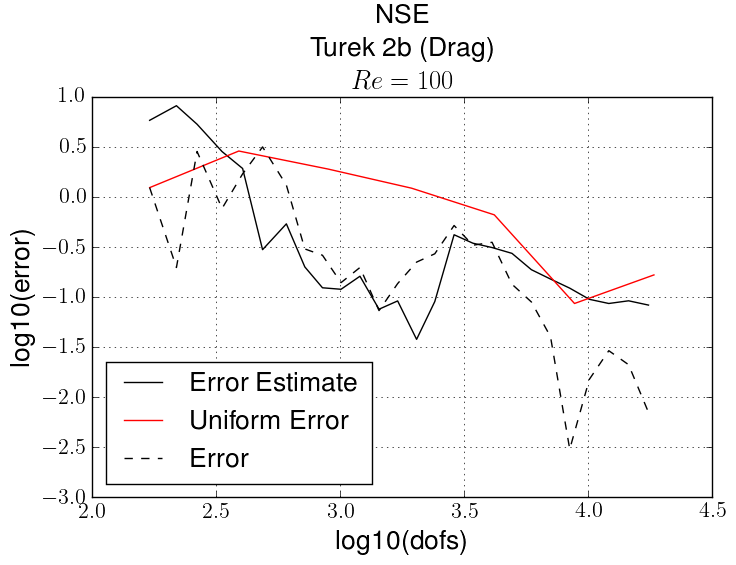
\includegraphics[scale=0.5]{Figures/AdaptiveNSEDragRe100.png}
        \caption{Adaptive error estimate versus ``true'' error for the solution
            for the NSE with Drag Functional.}
        \label{fig:NSEDrag_err}
    \end{figure}
\end{test}

\begin{test}[NSE, Velocity Functional] \label{tst:Velocity}
    For this test we choose the functional
    \begin{equation}
        M(\bar{U}^n) := \int_I\! \int_{\Omega}\! u\, d\mathbf{x}\, dt.
        \label{eq:VelocityFunctional}
    \end{equation}

    \begin{figure}[h]
        \centering
        \begin{minipage}[t]{0.49\textwidth}
            \centering
            \subcaptionbox{Initial mesh}{
                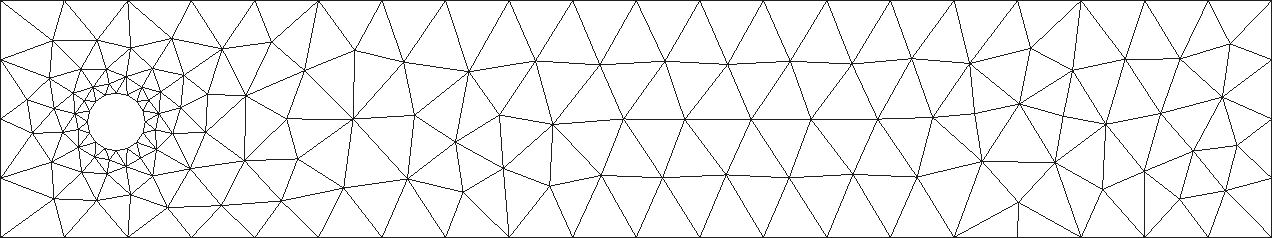
\includegraphics[scale=0.15]{Figures/AdaptiveNSEVelocityRe100_mesh0.png}
            }
            \subcaptionbox{Primal solution at $t=10$.}{
                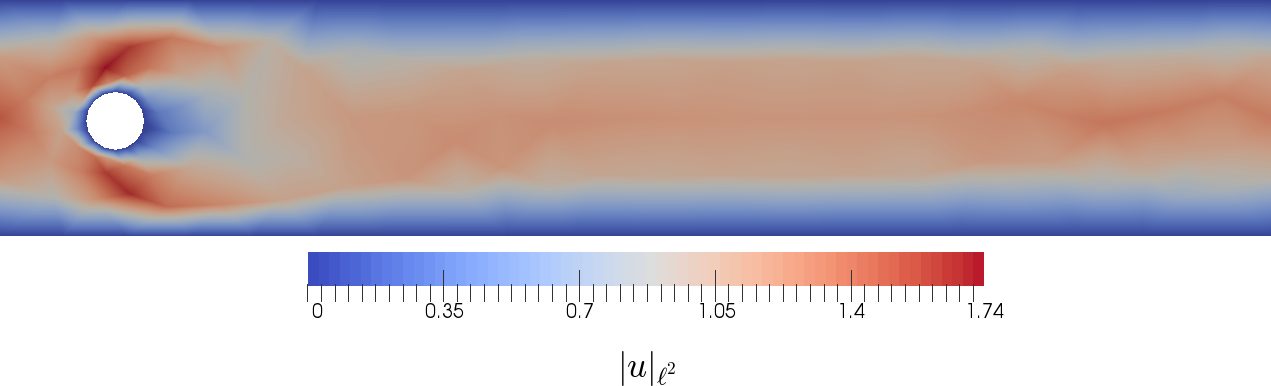
\includegraphics[scale=0.15]{Figures/AdaptiveNSEVelocityRe100_u0.png}
            }
            \subcaptionbox{Error indicators}{
                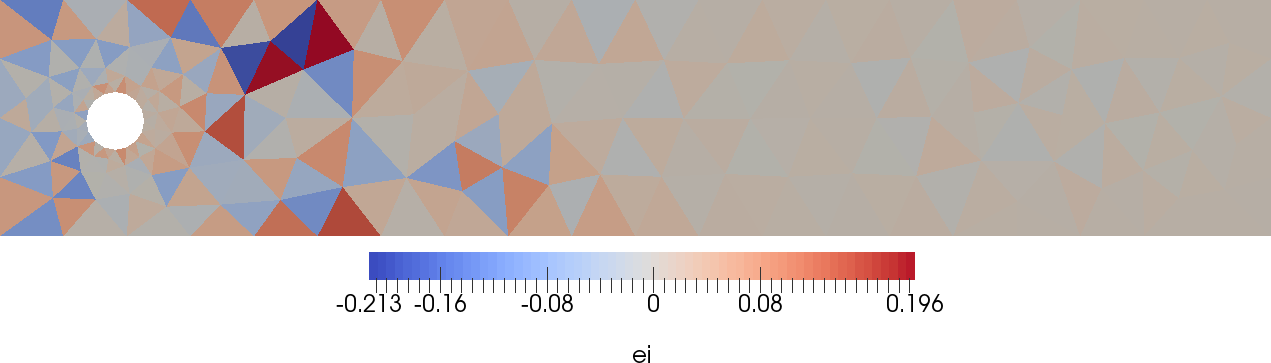
\includegraphics[scale=0.15]{Figures/AdaptiveNSEVelocityRe100_ei0.png}
            }
            \subcaptionbox{Dual solution at $t=0$.}{
                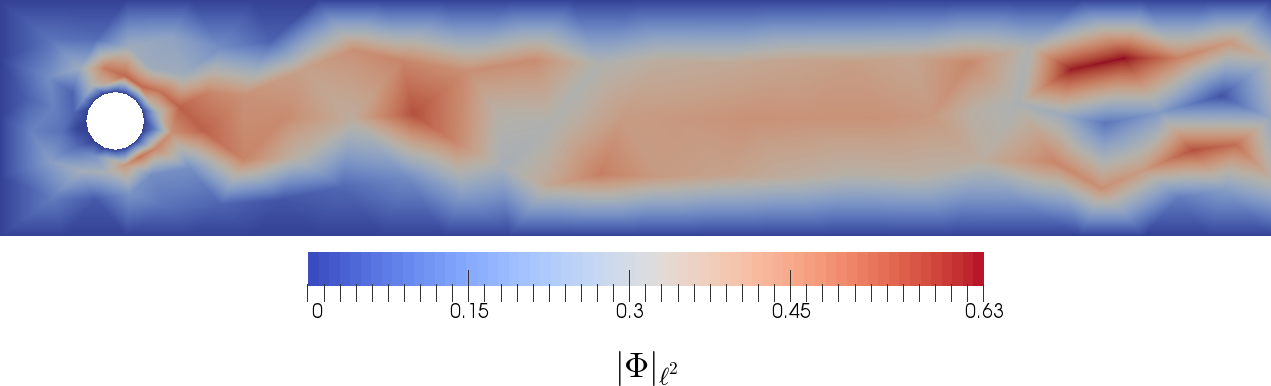
\includegraphics[scale=0.15]{Figures/AdaptiveNSEVelocityRe100_uDual0.png}
            }
        \end{minipage}
        \begin{minipage}[t]{0.49\textwidth}
            \centering
            \subcaptionbox{$25^{th}$ adaptive mesh}{
                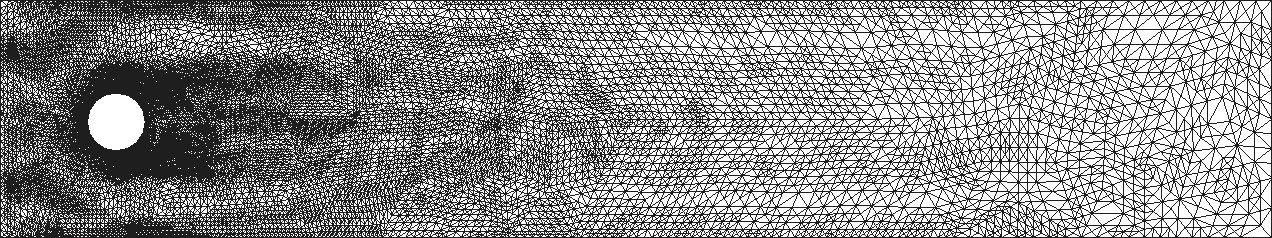
\includegraphics[scale=0.15]{Figures/AdaptiveNSEVelocityRe100_mesh25.png}
            }
            \subcaptionbox{Primal solution at $t=10$.}{
                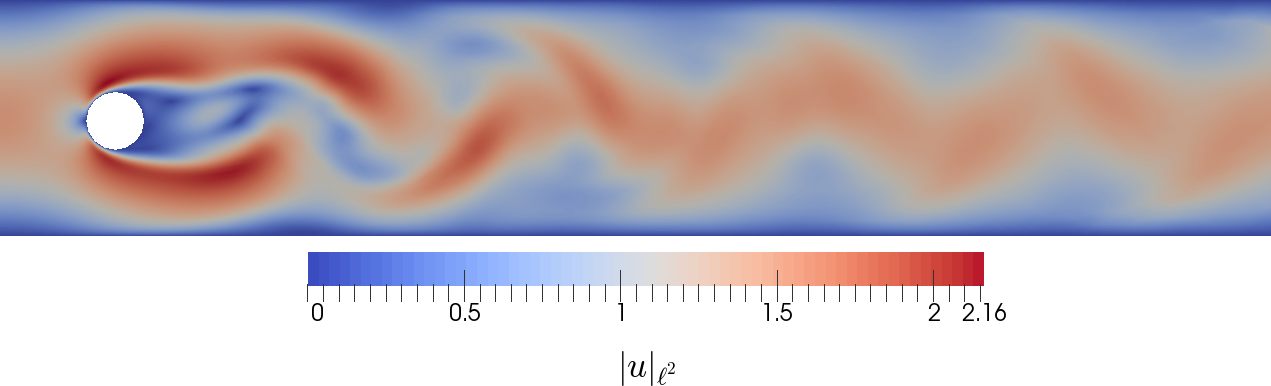
\includegraphics[scale=0.15]{Figures/AdaptiveNSEVelocityRe100_u25.png}
            }
            \subcaptionbox{Error indicators}{
                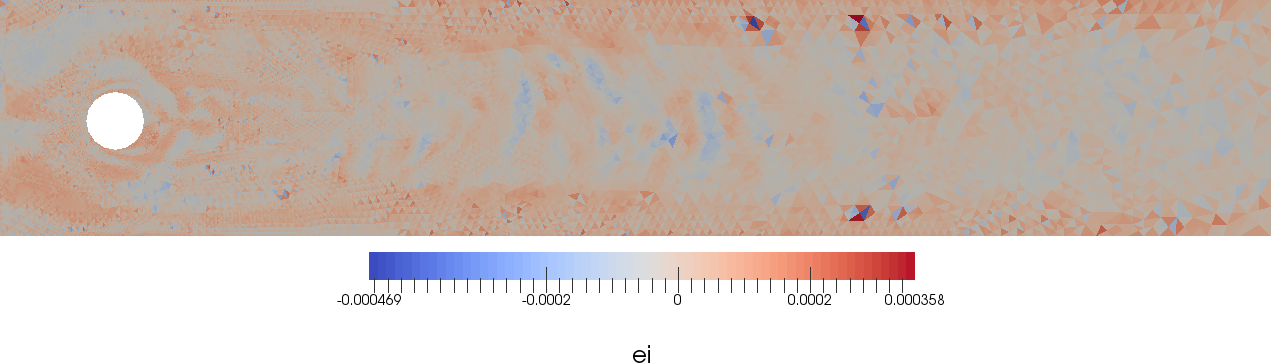
\includegraphics[scale=0.15]{Figures/AdaptiveNSEVelocityRe100_ei25.png}
            }
            \subcaptionbox{Dual solution at $t=0$.}{
                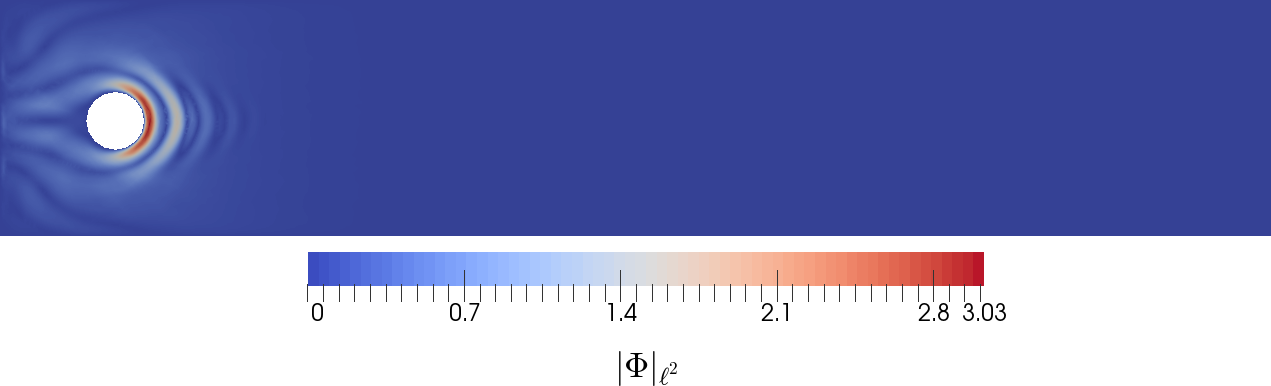
\includegraphics[scale=0.15]{Figures/AdaptiveNSEVelocityRe100_uDual25.png}
            }
        \end{minipage}
        \caption{Comparison of the Initial Mesh (Left), $170$ DOFs, to the
                 $25^{th}$ Adaptive mesh (Right), $20\, 183$ DoFs, for NSE with
                 Velocity Functional.}
    \end{figure}

    \begin{figure}[h]
        \centering
        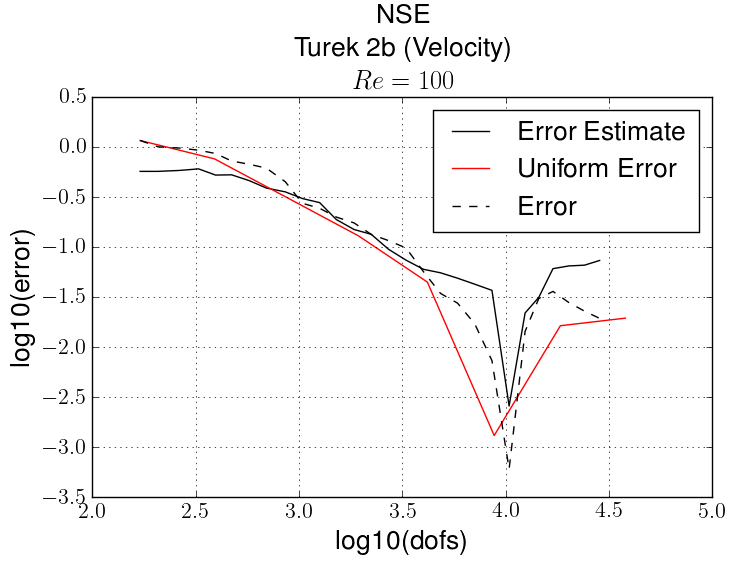
\includegraphics[scale=0.5]{Figures/AdaptiveNSEVelocityRe100.png}
        \caption{Adaptive error estimate versus ``true'' error for the solution
            for the NSE equation with Velocity Functional.}
        \label{fig:NSEVelocity_err}
    \end{figure}

\end{test}

\subsubsection{Variable Density Incompressible Navier-Stokes}

In this subsection we again will demonstrate the effectiveness of
\autoref{alg:Adaptivity}, but this time we apply the algorithm to a density
dependent problem. More specifically, in \autoref{tst:rhoNSE} we look at the
effectiveness of \autoref{alg:Adaptivity} applied to Rayleigh-Taylor instability
modelled by the variable density incompressible Navier-Stokes equations, i.e.
\begin{equation}
    \begin{split}
        &\rho_t + \nabla \cdot \left( \rho \mathbf{u} \right) = 0 \\
        &\rho \left( \mathbf{u}_t
            + \left( \mathbf{u}\cdot \nabla \right) \mathbf{u} \right)
            - \nu \Delta \mathbf{u} + \nabla p = \rho\, \mathbf{f} \\
        &\nabla \cdot \mathbf{u} = 0,
    \end{split}
    \label{eq:DensityNSE}
\end{equation}
where $\rho$ is the fluid density, $\mathbf{u} = \left[ u, v \right]^T$ is the
fluid velocity in 2D, $p$ is the fluid pressure, $\mathbf{f}$ is the
external forcing, and $\nu := \nicefrac{\mu}{\rho}$ is the kinematic viscosity,
which we will assume to be constant for these tests.

Again, we take a step size of $k$ and apply the $cG(1)cG(1)$finite
element to \autoref{eq:DensityNSE}, however this time we use a different
stabilization scheme. For the variable density Navier-Stokes equations we
choose to use artificial viscosity as our stabilization scheme. Thus, taking
$V = (v, q, \chi) \in X = \left[ H^1_0(\Omega) \right]^2 \times H^1(\Omega)
\times H^1(\Omega)$ results in the following weak residual
\begin{equation}
    \begin{split}
        r(\bar{U}^n; V) &= (\rho^n - \rho^{n-1}, \chi)
            + (\nabla \cdot \left( \bar{\rho}^n \bar{\mathbf{u}}^n \right), \chi) \\
        &\qquad+  \rho\, \left(\left(\mathbf{u}^n
                - \mathbf{u}^{n-1}, v\right)\,k^{-1}
            + (\left( \bar{\mathbf{u}}^n \cdot \nabla \right)
                \bar{\mathbf{u}}^n, v)\right) \\
        &\qquad+ \nu\, (\nabla \bar{\mathbf{u}}^n, \nabla v)
            + (\nabla p^n, v) - \rho\, (\mathbf{f}, v) \\
        &\qquad+ (\nabla \cdot \bar{\mathbf{u}}^n, v) = 0
    \end{split}
    \label{eq:WeakRhoNSE}
\end{equation}

\begin{test}[Rayleigh-Taylor Instability] \label{tst:rhoNSE}

    Variable density flows are valid for a wide range of natural phenomena such
    as, but not limited to: astrophysical flows, oceanic flows, atmospheric
    flows, and combustion. When the fluid is accelerated against the density
    gradient fluid instability is generated and small perturbations in the fluid
    interface grow and interact non-linearly resulting in turbulence.  This
    process is known as Rayleigh-Taylor (RT) instability and will be the focus of
    this particular test.

    For RT flows the primary non-dimensional parameter characterizing
    differential acceleration effects is the Atwood number:
    \begin{equation}
        A := \frac{\rho_2 - \rho_1}{\rho_2 + \rho_1}.
        \label{eq:Atwood}
    \end{equation}
    Thus for $\rho_1 = 1$ and $\rho_2 = 3$ the corresponding Atwood number would
    be $A = 0.5$. In addition to the Atwood number we can define two additional
    non-dimensional parameters, such as the Reynolds number, $Re$, and the
    Froude number, $Fr$:
    \begin{equation}
        Re = \frac{L U}{\nu}, \qquad Fr = \frac{U}{\sqrt{g\, L}},
        \label{eq:Re+Fr}
    \end{equation}
    where $g$ is the acceleration due to gravity, $L$ is the characteristic
    wavelength, $U$ is the reference velocity, $\nu$ again is the kinematic
    viscosity. With these scales defined as above we can then define the
    characteristic time scale, $\tau = \sqrt{\nicefrac{L}{(A\, g)}}$.

    For this test we must be careful when choosing our goal functional. Certain
    functionals may provide no useful information. For this reason we choose the
    following functional
    \begin{equation}
        M(\bar{U}^n) := \int_I\! \int_{\Omega}\! u + v\, d\mathbf{x}\, dt,
        \label{eq:FunctionalRhoNSE}
    \end{equation}
    which was shown to be as effective as $\int_I \int_{\Omega} \rho\,
    d\mathbf{x}\, dt$ in \cite{Izarra2014}. This is important since the scheme
    above is mass preserving and thus no information is gained from the density
    functional.

\end{test}
